%
% ---------------------------------------------------
%
% Trabajo Fin de Grado:
% Author: Laura Padrón Jorge <gonzalezsuarezivan@gmail.com>
% Author: F. de Sande fsande@ull.es
% Fichero: main.tex
%
% ----------------------------------------------------
%
\documentclass[spanish,a4paper,12pt,oneside]{extreport}
%\documentclass[a4paper, twoside, 12pt]{book}
\usepackage[a4paper]{geometry}
\usepackage[spanish]{babel}
\usepackage[utf8]{inputenc}
%\usepackage{lscape}
\usepackage{pdflscape}
%%%%%%%%%%%%%%%%%%%%%%%%%%%%%%%%%%%%%%%%%%%%%%%%%%%%%%%%%%%%%%%%%%%%%%%%%%%%%%%%%%%%%%%%%%%%
% Next 3+3 lines select PDF or PS output (comment as apropriate)
% To switch from PDF and PS comment/uncomment here and change Makefile
\usepackage[pdftex]{color}
\usepackage[pdftex]{graphicx}
\graphicspath{{images/}}
%\usepackage[dvips]{color}
%\usepackage[dvips]{graphicx}
\usepackage{epsfig}
%\graphicspath{{images/eps/}}
%Añadidos BulletPoint
\usepackage{floatrow}
%%%%%%%%%%%%%%%%%%%%%%%%%%%%%%%%%%%%%%%%%%%%%%%%%%%%%%%%%%%%%%%%%%%%%%%%%%%%%%%%%%%%%%%%%%%%
\usepackage{algorithmic}
\usepackage[pdftex=true,colorlinks=false,urlcolor=blue,plainpages=false,pagebackref=true,citecolor=red]{hyperref} %hiperenlaces y backcites 
%%%%%%%%%%%%%%%%%%%%%%%%%%%%%%%%%%%%%%%%%%%%%%%%%%%%%%%%%%%%%%%%%%%%%%%%%%%%%%%%%%%%%%%%%%%%
% Comandos para escribir "siempre igual"
\newcommand{\BulletP}{\texttt{BulletPoint.{ Tecnología beacon en entornos universitarios}}}

\newcommand{\llCoMP}{\texttt{llCoMP}{}}
\newcommand{\BulletPoint}{\texttt{BulletPoint}{}}


%%% Traducimos el pseudocodigo
\renewcommand{\algorithmicwhile}{\textbf{mientras}}
\renewcommand{\algorithmicend}{\textbf{fin}}
\renewcommand{\algorithmicdo}{\textbf{hacer}}
\renewcommand{\algorithmicif}{\textbf{si}}
\renewcommand{\algorithmicthen}{\textbf{entonces}}
\renewcommand{\algorithmicrepeat}{\textbf{repetir}}
\renewcommand{\algorithmicuntil}{\textbf{hasta que}}
\renewcommand{\algorithmicelse}{\textbf{en otro caso}}
\renewcommand{\algorithmicfor}{\textbf{para}}

%%%%%%%%%%%%%%%%% Creamos un entorno para listar código fuente %%%%%%%%%%%%%%%
\newenvironment{sourcecode}
{\begin{list}{}{\setlength{\leftmargin}{1em}}\item\scriptsize\bfseries}
{\end{list}}

\newenvironment{littlesourcecode}
{\begin{list}{}{\setlength{\leftmargin}{1em}}\item\tiny\bfseries}
{\end{list}}

\newenvironment{summary}
{\par\noindent\begin{center}\textbf{Abstract}\end{center}\begin{itshape}\par\noindent}
{\end{itshape}}

\newenvironment{keywords}
{\begin{list}{}{\setlength{\leftmargin}{1em}}\item[\hskip\labelsep \bfseries Keywords:]}
{\end{list}}

\newenvironment{palabrasClave}
{\begin{list}{}{\setlength{\leftmargin}{1em}}\item[\hskip\labelsep \bfseries Palabras clave:]}
{\end{list}}


%%%%%%%%%%%%%%%%%%%%%%%%%%%%%%%%%%%%%%%%%%%%%%%%%%%%%%%%%%%%%%%%%%%%%%%%%%%%%%%
\definecolor{marron}       {rgb}{0.496, 0.203, 0.152}
\definecolor{verde-claro}  {rgb}{0.625, 0.734, 0.199}
\definecolor{oscuro}       {rgb}{0.187, 0.141, 0.285}
\definecolor{gris}     	   {rgb}{0.500, 0.500, 0.500}
\definecolor{bgd-listings} {rgb}{0.999, 0.999, 0.900}
\definecolor{gray97}{gray}{.97}
\definecolor{gray75}{gray}{.75}
\definecolor{gray45}{gray}{.45}
\definecolor{gray}{gray}{.45}
%%%%%%%%%%%%%%%%%%%%%%%%%%%%%%%%%%%%%%%%%%%%%%%%%%%%%%%%%%%%%%%%%%%%%%%%%%%%%%%%%%%%%%%%%%%%
%%% Code Listings
%\usepackage{listings} 
%\lstloadlanguages{python,C}
\definecolor{Brown}{cmyk}{0,0.81,1,0.60}
\definecolor{OliveGreen}{cmyk}{0.64,0,0.95,0.40}
\definecolor{CadetBlue}{cmyk}{0.62,0.57,0.23,0}
\definecolor{lightlightgray}{gray}{0.9}
%%%%%%%%%%%%%%%%%%%%%%%%%%%%%%%%%%%%%%%%%%%%%%%%%%%%%%%%%%%%%%%%%%%%%%%%%%%%%%%%%%%%%%%%%%%
%Evitar partir palabras al final de la línea
\hyphenpenalty=10000
\tolerance=1000
%%%%%%%%%%%%%%%%%%%%%%%%%%%%%%%%%%%%%%%%%%%%%%%%%%%%%%%%%%%%%%%%%%%%%%%%%%%%%%%%%%%%%%%%%%%%
% Para listados de código
\usepackage{listings}
\lstloadlanguages{C}

% Definiendo colores para los listados de código fuente - Univ. Deusto
\definecolor{violet}{rgb}{0.5,0,0.5}
\definecolor{navy}{rgb}{0,0,0.5}
\definecolor{hellgelb}{rgb}{1,1,0.8}
\definecolor{colKeys}{rgb}{0,0,1}
\definecolor{colIdentifier}{rgb}{0,0,0}
\definecolor{colComments}{rgb}{1,0,0}
\definecolor{colString}{rgb}{0,0.5,0}

%\lstset{morekeywords={pragma copy\_in copy\_out copy omp parallel private reduction shared hicuda loop\_partition over\_tblock over\_thread}}
\lstset{
        float=tbhp,
		    language = Java,
				morekeywords={llc,reduction_type,nc_result,
				              hicuda,global,alloc,shape,kernel,thread,loop_partition,tblock,over_tblock,over_thread,kernel_end,copyout,free,
											data,region,
											task,input,inout,output,
				              pragma,omp,parallel,reduction,private,shared,target,device,copy_in,copy_out,
				              acc,kernels,loop,copyin,copy,pcopy,pcopyin,collapse,gang,worker,independent},
				%\emph      ={omp,parallel,reduction,private,shared},
				emphstyle=\textbf,
        %basicstyle=\ttfamily\tiny,
        basicstyle=\ttfamily\scriptsize,
        identifierstyle=\color{colIdentifier},
        keywordstyle=\color{colKeys},
        stringstyle=\color{colString},
        commentstyle=\color[rgb]{0.133,0.545,0.133},
        columns=flexible,
        tabsize=4,
        frame=single,
        extendedchars=true,
        showspaces=false,
        showstringspaces=false,
        numbers=left,
        numberstyle=\tiny,
        breaklines=true,
        backgroundcolor=\color{lightlightgray},
        breakautoindent=true,
        captionpos=b
}

%\renewcommand{\lstlistingname}{Listing} % Los títulos de los códigos insertados se denotan con Ejemplo...   

% Otro formato más bonito para código fuente
\newcommand{\codigofuente}[3]{%
  \lstlisting[language=#1,caption={#2}]{#3}%
}
%%%%%%%%%%%%%%%%%%%%%%%%%%%%%%%%%%%%%%%%%%%%%%%%%%%%%%%%%%%%%%%%%%%%%%%%%%%%%%%
\begin{document}
\renewcommand{\lstlistingname}{Listado}% Listing -> Listado de código
%%%%%%%%%%%%%%%%%%%%%%%%%%%%%%%%%%%%%%%%%%%%%%%%%%%%%%%%%%%%%%%%%%%%%%%%%%%%%%%
% First Page
%%%%%%%%%%%%%%%%%%%%%%%%%%%%%%%%%%%%%%%%%%%%%%%%%%%%%%%%%%%%%%%%%%%%%%%%%%%%%%%

\pagestyle{empty}
\thispagestyle{empty}


\newcommand{\HRule}{\rule{\linewidth}{1mm}}
\setlength{\parindent}{0mm}
\setlength{\parskip}{0mm}

\vspace*{\stretch{0.5}}

\begin{center}

\includegraphics[scale=0.8]{images/logo_vertical}\\[10mm]
{\Huge Trabajo de Fin de Grado}
\end{center}

\HRule
\begin{flushright}
        {\Huge \BulletP{}} \\[2.5mm]
        {\Large Laura Padrón Jorge} \\[5mm]


\end{flushright}
\HRule
\vspace*{\stretch{2}}
\begin{center}
  \Large La Laguna, \today
\end{center}

\setlength{\parindent}{5mm}

%%%%%%%%%%%%%%%%%%%%%%%%%%%%%%%%%%%%%%%%%%%%%%%%%%%%%%%%%%%%%%%%%%%%%%%%%%%%%%%
% Signature page (add the official stamp)
%%%%%%%%%%%%%%%%%%%%%%%%%%%%%%%%%%%%%%%%%%%%%%%%%%%%%%%%%%%%%%%%%%%%%%%%%%%%%%%
\newpage
%\cleardoublepage
\thispagestyle{empty}

D. {\bf Francisco de Sande González}, con DNI nº 42.067.050-G
profesor
Titular de Universidad
adscrito al Departamento
de Ingeniería Informática y de Sistemas
de la Universidad de La Laguna, como tutor

\bigskip

\bigskip
\bigskip
{\bf C E R T I F I C A}

\bigskip
\bigskip
\bigskip
Que la presente memoria titulada:

\bigskip
``{\it \BulletP{}}''

\bigskip
\bigskip
\bigskip
%Cambiar
\noindent ha sido realizada bajo su dirección por D.ª {\bf Laura Padron Jorge},
con DNI nº 79.089.251-W

\bigskip
\bigskip

Y para que así conste, en cumplimiento de la legislación vigente y a los efectos
oportunos firman la presente en La Laguna a \today

%\cleardoublepage
\newpage
%%%%%%%%%%%%%%%%%%%%%%%%%%%%%%%%%%%%%%%%%%%%%%%%%%%%%%%%%%%%%%%%%%%%%%%%%%%%%%%
\thispagestyle{empty}

{ \flushright

\begin{LARGE}
Agradecimientos
\end{LARGE}

\hspace{3mm}

\begin{large}


\hspace{3mm}

Mis agradecimientos al profesor Francisco de Sande González por su labor como tutor de este proyecto, orientando este trabajo, compartiendo su conocimiento y exigiendo siempre lo mejor. 

Asimismo, me gustaría agradecer a la Universidad de La Laguna, a los Servicios TIC y a Don Juan Carlos Hernández Perdomo de los servicios TIC de la ULL su colaboración en este proyecto y la puesta a disposición de los beacons, sin los cuáles habría sido imposible el desarrollo de este proyecto. 

Gracias a Don Alberto Morales de la empresa Galotecnia Redes Sistemas y Servicios SL, por su tiempo y dedicación en la explicación de los requisitos técnicos necesarios para la implantación de los beacons en el sistema de parking de la ULL, de estudio en el desarrollo de este trabajo.

Por último, agradecer también al personal de TITSA por el trato recibido, la participación y la rápida respuesta a las consultas, facilitando con ello el desarrollo del proyecto.


\end{large}

}

%%%%%%%%%%%%%%%%%%%%%%%%%%%%%%%%%%%%%%%%%%%%%%%%%%%%%%%%%%%%%%%%%%%%%%%%%%%%%%%%%
\newpage

\begin{huge}
Licencia
\end{huge}

\bigskip
%* Si quiere permitir que se compartan las adaptaciones de tu obra mientras se comparta de la misma manera
%y NO quieres permitir usos comerciales de tu obra indica:

\begin{center}

\includegraphics[scale=1.5]{images/by-nc-sa_88x31}\\[10mm]
{\Large \copyright~Esta obra está bajo una licencia de Creative Commons Reconocimiento-NoComercial-CompartirIgual 4.0 Internacional.
}
\end{center}


%%%%%%%%%%%%%%%%%%%%%%%%%%%%%%%%%%%%%%%%%%%%%%%%%%%%%%%%%%%%%%%%%%%%%%%%%%%%%%%
\newpage  %\cleardoublepage
\begin{abstract}
{\em

Este documento constituye el trabajo de investigación de la alumna durante el proceso de desarrollo de una aplicación para dispositivos móviles Android mediante el uso de una de las tecnologías más recientes y menos conocidas en el mercado actual: los Beacons.

\bigskip
Partimos de los conocimientos de programación en \textit{Java} adquiridos en la asignatura: \textit{``Diseño arquitectónico y patrones''} cursada en el 
itinerario de Ingeniería del Software. Esta asignatura, impartida en el tercer curso del Grado en Ingeniería Informática de la Universidad de La Laguna, ha sido la que ha sentado los fundamentos a partir de los cuáles se ha desarrollado la aplicación.

\bigskip
Durante este proyecto, la alumna ha conseguido adquirir independencia en su trabajo, visión y planificación realizando tareas de investigación, desarrollo y documentación, que han dado como resultado la obtención de conocimientos durante el proceso de trabajo.

\bigskip 
También se ha investigado la reciente tecnología ``beacon'' que si bien aún no tiene un impacto muy grande, en un futuro inmediato se espera que se empiece a utilizar con naturalidad en distintos ámbitos: turismo, comercio, enseñanza, etc.

}
\begin{palabrasClave}
Aplicaciones Android, Java, dispositivos móviles, programación, Beacons.
\end{palabrasClave}

\end{abstract}
%%%%%%%%%%%%%%%%%%%%%%%%%%%%%%%%%%%%%%%%%%%%%%%%%%%%%%%%%%%%%%%%%%%%%%%%%%%%%%%

%%%%%%%%%%%%%%%%%%%%%%%%%%%%%%%%%%%%%%%%%%%%%%%%%%%%%%%%%%%%%%%%%%%%%%%%%%%%%%%
\newpage  %\cleardoublepage
\begin{summary}
{\em

The aim of the project has been the development of an application for Android devices that uses beacon technology for some of its main features.

\bigskip
Based on the knowledge of \textit{Java} programming obtained in the subject: \textit{``Architectural Design and Patterns''} studied in the
Software Engineering Branch (given in third year of Computing Engineering degree from \textit{``La Universidad de La Laguna''}). In this work we have acquired the basic knowledge needed to develop Android applications introducing us in the development of applications related to beacon technology.

\bigskip
Moreover, the student has learned independence in her work and gained vision and scheduling aptitudes, developing different labors of research, development and documentation that have come to give her a wide knowledge during the development of this project.

\bigskip
Apart from all this, it's of great value for the student to get to know this new beacon technology. I have investigated and learned from this new technology, which at the moment is not well known, but in the close future it is expected to get more attention in different sectors, such as tourism, trading or learning.
}

\begin{keywords}
Application for Android, Java, mobile devices, programming, Beacons.
\end{keywords}

\end{summary}
%%%%%%%%%%%%%%%%%%%%%%%%%%%%%%%%%%%%%%%%%%%%%%%%%%%%%%%%%%%%%%%%%%%%%%%%%%%%%%%

%%%%%%%%%%%%%%%%%%%%%%%%%%%%%%%%%%%%%%%%%%%%%%%%%%%%%%%%%%%%%%%%%%%%%%%%%%%%%%%
\newpage{\pagestyle{empty}}
\thispagestyle{empty}

%%%%%%%%%%%%%%%%%%%%%%%%%%%%%%%%%%%%%%%%%%%%%%%%%%%%%%%%%%%%%%%%%%%%%%%%%%%%%%%


\pagestyle{myheadings} %my head defined by markboth or markright
% No funciona bien \markboth sin "twoside" en \documentclass, pero al
% ponerlo se dan un montón de errores de underfull \vbox, con lo que no se
% ha puesto.
\markboth{Laura Padrón Jorge}{BulletPoint}

%%%%%%%%%%%%%%%%%%%%%%%%%%%%%%%%%%%%%%%%%%%%%%%%%%%%%%%%%%%%%%%%%%%%%%%%%%%%%%%
%Numeracion en romanos
\renewcommand{\thepage}{\roman{page}}
\setcounter{page}{1}

%%%%%%%%%%%%%%%%%%%%%%%%%%%%%%%%%%%%%%%%%%%%%%%%%%%%%%%%%%%%%%%%%%%%%%%%%%%%%%%

\tableofcontents

%%%%%%%%%%%%%%%%%%%%%%%%%%%%%%%%%%%%%%%%%%%%%%%%%%%%%%%%%%%%%%%%%%%%%%%%%%%%%%%
\newpage{\pagestyle{empty}}

\listoffigures

%%%%%%%%%%%%%%%%%%%%%%%%%%%%%%%%%%%%%%%%%%%%%%%%%%%%%%%%%%%%%%%%%%%%%%%%%%%%%%%
\newpage{\pagestyle{empty}}

%\listoftables

%%%%%%%%%%%%%%%%%%%%%%%%%%%%%%%%%%%%%%%%%%%%%%%%%%%%%%%%%%%%%%%%%%%%%%%%%%%%%%%
\newpage{\pagestyle{empty}}

%%%%%%%%%%%%%%%%%%%%%%%%%%%%%%%%%%%%%%%%%%%%%%%%%%%%%%%%%%%%%%%%%%%%%%%%%%%%%%%
%Numeracion a partir del capitulo I
\renewcommand{\thepage}{\arabic{page}}
\setcounter{page}{1}


% ==========================================================
% --------               Capítulos                ----------
% --------    Estan en el directorio capitulos/   ----------
% ==========================================================
% ---------------------------------------------------
%
% Proyecto de Final de Carrera: 
% Author: Laura Padron Jorge <alu0100703511@ul.edu.es>
% Introducción
% Fichero: Prologo.tex
%
% ----------------------------------------------------

\chapter*{Introducción}
\addcontentsline{toc}{chapter}{Introducción} 

Este documento comprende el trabajo de investigación y desarrollo realizado por la alumna en la consecución de su Trabajo de Fin de Grado (TFG), con el que culminará sus estudios del Grado en Ingeniería Informática cursados en la Escuela Superior de Ingeniería y Tecnología (ESIT) de la Universidad de la Laguna (ULL).

%
% ---------------------------------------------------
%
% Proyecto de Final de Carrera:
% Author: Laura Padrón Jorge <alu0100703511@ull.edu.es>
% Capítulo: Objetivos 
% Fichero: Cap1_Goals.tex
%
% ----------------------------------------------------
%


\chapter{Objetivos} \label{chap:Objetivos}  

Este TFG tiene los siguientes objetivos principales:

	
\begin{itemize}
\item  	Por un lado se pretende ampliar los conocimientos en tecnologías móviles en el sistema operativo \textit{Android} \cite{URL::Android} y en el desarrollo de aplicaciones para este sistema operativo.
\item Por otro lado, también se pretende que la alumna se familiarice con el uso de herramientas de control de versiones utilizando GitHub \textit{Github} \cite{URL::Github} y de edición de textos técnicos utilizando \textit{LaTeX}  \cite{URL::LaTeX}.
\item Otro objetivo presente en este TFG es que la alumna investigue y profundice en una tecnología reciente en el mercado, los \textit{Beacons} \cite{URL::Beacon}.
\item  Por último, se espera que la estudiante obtenga independencia en su trabajo, visión y planificación poniendo en marcha tareas de investigación, documentación, desarrollo y despliegue utilizando tanto los conocimientos adquiridos durante la carrera, como aquellos que se irán aprendiendo durante el progreso de este trabajo.
\end{itemize}
% ---------------------------------------------------
%
% Trabajo de Fin de Grado. 
% Author: Laura Padrón Jorge. 
% Capítulo: Tecnologías utilizadas en el Trabajo de Fin de Grado. 
% Fichero: Cap2_Technology.tex
%
% ----------------------------------------------------
%

\cleardoublepage
\chapter{Herramientas y Tecnologías utilizadas} \label{chap:Tecnologias} 

Este capítulo tiene como objetivo presentar las distintas herramientas software y tecnologías empleadas por la alumna en el desarrollo de este trabajo.

\section{Herramientas de Desarrollo}

A continuación se explicarán brevemente las distintas herramientas software utilizadas en el proyecto. 

\subsection{Android Studio}

Android Studio \cite{URL::AndroidStudio} es el IDE (Entorno de Desarrollo Integrado) oficial para el desarrollo de aplicaciones en Android, basado en IntelliJ IDEA \cite{URL::IntelliJIDEA}. Android Studio ofrece una serie de funcionalidades que han facilitado a la desarrolladora numerosas tareas, entre las cuales podemos destacar:


\begin{itemize}
\item Un sistema de compilación basado en Gradle\cite{URL::Gradle} que ha simplificado tanto la inserción de dependencias de las distintas librerías que se han tenido que utilizar, como la compilación de la aplicación.
\item Un emulador rápido y fácil de utilizar que ha ayudado a visualizar las distintas pantallas durante el desarollo aunque no ha sido de mucha utilidad para probar el funcionamiento al ser dependiente la app de la tecnología Bluetooth.
\item La facilidad para publicar cambios a aplicaciones ya funcionando sin tener que eliminar y volver a crear un nuevo APK parando la app.
\item Un sistema de visualización de las diferentes pantallas muy completo, con soporte visual para añadir componentes y cambiar atributos fácilmente.
\item Un sistema de depuración, con una interfaz sencilla e intuitiva.
\end{itemize} 

\begin{figure}[h]
	\centering
	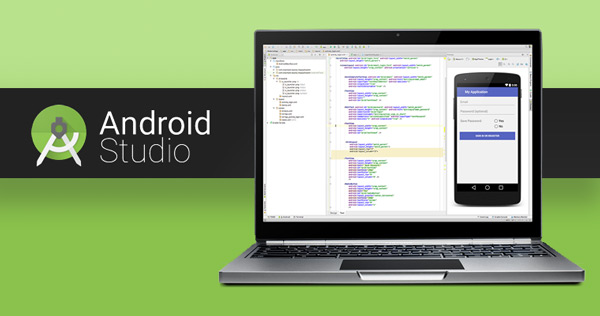
\includegraphics[width=\linewidth]{androidstudio}
	\caption{Android Studio, un IDE flexible e intuitivo.}
	\label{fig:androidstudio}
\end{figure}

Se ha utilizado este IDE frente a otros como Eclipse + ADT \cite{URL::eclipseADT} debido a que en la actualidad es el IDE oficial con soporte de Google. Se ha preferido aprender a utilizar este entorno con vistas al futuro, ya que parece que se consolidará como el preferido para los desarrolladores Android.

\subsection{LaTex}

LaTeX \cite{URL::LaTeX} es un sistema de composición de textos, orientado a la creación de documentos que presenten una alta calidad tipográfica. Por sus características y posibilidades, es usado especialmente en la generación de artículos y publicaciones científicas que incluyen, entre otros elementos, expresiones matemáticas, gráficos o figuras.


LaTeX está formado por un gran conjunto de macros de TeX, escrito por Leslie Lamport en 1984, con la intención de facilitar el uso del lenguaje de composición tipográfica, creado por Donald Knuth. LaTeX es software libre bajo licencia LPPL.


Se ha decidido utilizar este sistema debido al carácter profesional que aporta a los documentos. Ha sido una buena oportunidad para aprender a usar un sistema de composición de texto como este, ya que en un futuro puede ser beneficioso el saber manejar esta herramienta. 


Si bien es cierto, que el uso de esta herramienta frente a otros editores más familiares ha sido algo tedioso en el inicio, es verdad que una vez acostumbrada a su uso ha resultado ser muy eficaz. En el proceso de aprendizaje se recurrió principalmente a manuales por internet, alguno a destacar en español sería \cite{URL::manualLatex}

\subsection{Github}

GitHub\cite{URL::Github} es una forja (plataforma de desarrollo colaborativo) para alojar proyectos que utiliza el sistema de control de versiones Git. Utiliza el framework Ruby on Rails por GitHub, Inc. (anteriormente conocida como Logical Awesome). Desde enero de 2010, GitHub opera bajo el nombre de GitHub, Inc. El código se almacena de forma pública, aunque también se puede hacer de forma privada, creando una cuenta de pago.


Se ha decidido crear un repositorio en esta plataforma para poder llevar un control y una trazabilidad del proyecto. El tutor y la alumna han trabajado en este repositorio de manera conjunta. En el caso del tutor, principalmente para revisar el seguimiento semanal y llevar un control de las tareas. En el caso de la alumna, para tener un repositorio donde subir los distintos elementos que se han ido generando a lo largo del trabajo. Aparte de este repositorio, también se ha abierto un segundo repositorio \cite{URL::repositorioAplicacion} asociado a la oficina del software libre (OSL) para subir el código una vez terminado como parte del programa de apoyo a trabajos finales libres (PATFL) \cite{URL::PATFL} de la ULL.


Mediante el uso de este repositorio, la alumna ha conseguido ampliar sus conocimientos en Git y familiarizarse con la interfaz de GitHub. Previamente se había utilizado como repositorios GitLab, SVN y RTC en otros proyectos, por lo que no ha sido una complicación mayor utilizar este sistema.

\section{Tecnologías utilizadas}

A continuación se revisan las distintas tecnologías utilizadas en el desarrollo de la aplicación.

\subsection{El Sistema Operativo Android}

Android es un sistema operativo que emplea Linux en la interfaz del hardware.  Los componentes del SO subyacentes se codifican en C o C++ pero las aplicaciones se desarrollan en Java. De esta manera Android asegura una amplia operatividad en una gran variedad de dispositivos debido a dos hechos: la interfaz en Linux ofrece gran potencia y funcionalidad para aprovechar el hardware, mientras que el desarrollo de las aplicaciones en Java permite que Android sea accesible para un gran número de programadores conocedores del código.

Este SO fue diseñado principalmente para dispositivos móviles con pantalla táctil: smartphones, tablets y otros dispositivos como televisores o automóviles. Fue desarrollado inicialmente por Android Inc., empresa que fue respaldada económicamente por Google y más tarde aquirida por esta misma empresa.

Actualmente tiene una gran comunidad de desarrolladores creando aplicaciones para extender la funcionalidad de los dispositivos. A fecha de hoy existen más de un millón de aplicaciones disponibles para la tienda oficial de Apps de Android, Google Play \cite{URL::GooglePlay} sin tener en cuenta las aplicaciones de otras tiendas no oficiales, como por ejemplo, la tienda de aplicaciones de Samsung Apps \cite{URL::SamsungApps}.

\subsection{Los Beacons}

Los \textit{''Beacons''} \cite{URL::Beacon} (la traducción del término sería a \textit{'balizas'} o \textit{'faros'}) son una tecnología emergente que desde hace algunos años se intenta abrir paso en el mercado. Como su propio nombre indica, estos dispositivos intentan ser un mecanismo de guía, dando una solución al posicionamiento en interiores, donde otras tecnologías, como el GPS \cite{URL::GPS} o el Wifi dejan de funcionar o resultan imprecisas. Sin embargo, estos no son los únicos usos de los beacons, actualmente muchas empresas están ampliando sus usos a otros campos.


A continuación se intentará responder a las preguntas más frecuentes que nos pueden surgir con respecto a esta tecnología:


\begin{itemize}
\item ¿Qué es un beacon?
\item ¿Cómo funcionan estos dispositivos?
\item ¿Qué rango de alcance poseen?
\item ¿Con qué dispositivos móviles son compatibles? 
\item ¿Qué ventajas y desventajas tienen con respecto a otras tecnologías?
\item ¿Qué usos se le ha dado a esta tecnología hasta ahora?
\end{itemize}

\begin{figure}[!h]
        \begin{floatrow}
        \ffigbox{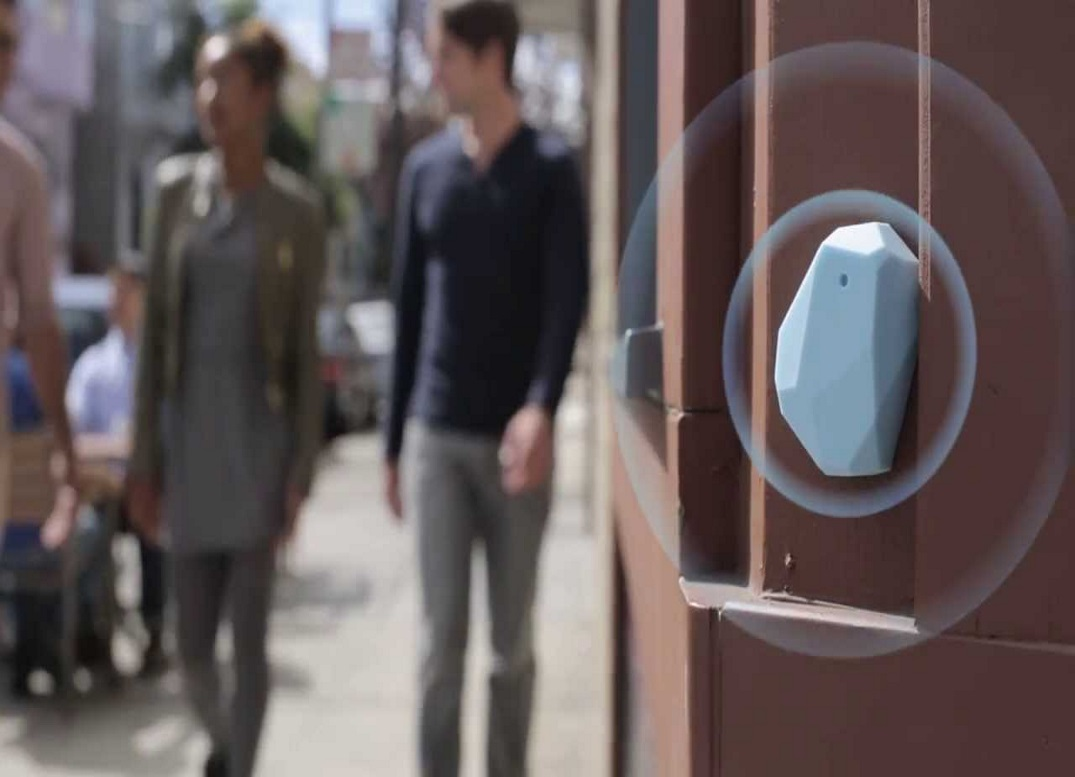
\includegraphics[width=\textwidth/2]{estimoteBeacon}}{\caption{Uno de los beacons de la compañia Estimote}\label{fig:estimote_Beacon}}
        \ffigbox{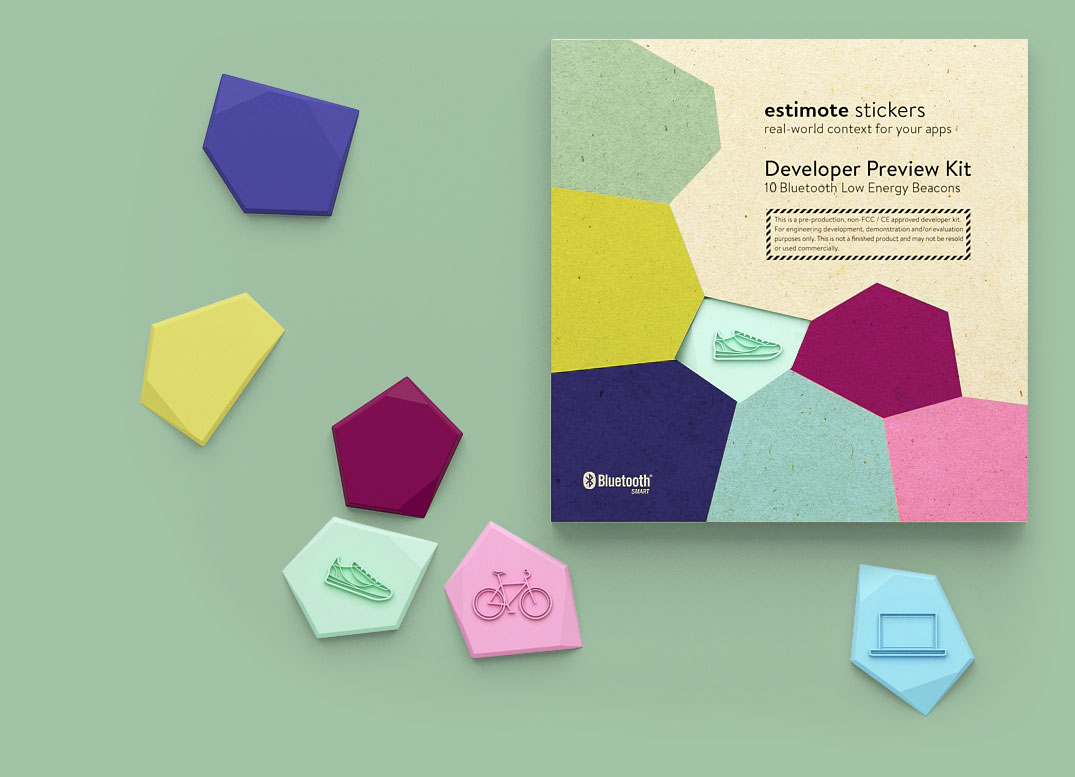
\includegraphics[width=\textwidth/2]{estimoteSticker}}{\caption{Uno de los beacons de la compañia Estimote en formato Pegatina}\label{fig:estimote_Beacon_Sticker}}
        \end{floatrow}
\end{figure}

\subsubsection{¿Qué es un Beacon?}

Para quienes no conozcan este término, en el marco en el que nos movemos, hace referencia a un pequeño dispositivo (sus tamaños varían de uno a otro, pero siempre de tamaño reducido) que emite señales de onda corta utilizando la tecnología Bluetooth \cite{URL::Bluetooth}. Estas señales contienen una pequeña cantidad de información que es recibida por dispositivos móviles con tecnología Bluetooth dentro de un rango de cobertura variable dependiendo del beacon y su configuración. Normalmente, la intensidad de esta señal y su frecuencia son configurables.

\begin{figure}[h]
	\centering
	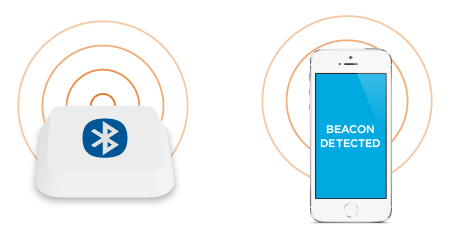
\includegraphics[width=\linewidth]{beaconPhone}
	\caption{Representación de un beacon emitiendo mediante Bluetooth a un dispositivo móvil}
	\label{fig:beaconBluetooth}
\end{figure}

El funcionamiento de un beacon es sencillo: El dispositivo emite una señal ininterrumpida (Véase Figura \ref{fig:beaconBluetooth}) que es captada por los dispositivos móviles dentro de su radio de cobertura. La señal nos ofrece información que sirve para detectar y localizar estos dispositivos. Esta señal es captada por una aplicación previamente instalada en un dispositivo móvil que esté programada para recibirla y reaccionar de manera acorde a la información recibida.


Hay que tener en cuenta que esta señal es unidireccional: los beacons son capaces de enviar pero no están preparados para recibir. También hay que tener en cuenta, que la mayoría de los beacon actuales en el mercado transmiten información preconfigurada, confiando en la aplicacion móvil para utilizar la información; sin embargo es muy posible que esto cambie en un futuro, ampliando las posibilidades de los beacons.

\subsubsection{¿Como funcionan estos dispositivos?}

Los beacons usan Bluetooth Low Energy (BLE) \cite{URL::BluetoothLowEnergy}, una versión del protocolo Bluetooth diseñada para usar mucha menos energía y enviar menos información. Los beacons funcionan con baterías cuyo tiempo de vida depende de la configuración establecida, teniendo en cuenta la emisión de la señal (intensidad y frecuencia) y tiempo de hibernación. Sus tiempos de vida son variables, pudiendo durar desde un mes hasta varios años. 

\begin{figure}[h]
	\centering
	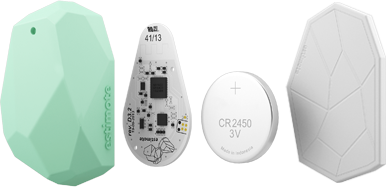
\includegraphics[width=0.7\linewidth]{estimoteBeaconInside}
	\caption{Interior de un beacon de Estimote}
	\label{fig:beaconInside}
\end{figure}

Independientemente de lo que se pueda pensar, los beacons en sí mismos no transmiten información significativa, transmiten identificadores cortos (a modo de información configurable), que son interpretados por una aplicación que sepa lo que ha de hacer cuando detecte esta información y que es la que se encarga de procesarla y realizar la acción pertinente.

Este identificador se divide en tres partes: 

\begin{itemize}
\item \textit{"`UUID"'} \cite{URL::UUID} : corresponde con una ID dada por el fabricante e identifica el beacon en cuestión, nosotros utilizaremos el término MAC para referirnos a este identificador. \label{el:mac}
\item ID Superior : configurables y utilizadas con un significado específico que puede identificar una acción o parámetro. 
\item ID Inferior: customconfigurablesizables y utilizadas al igual que la superior con un significado específico que se puede usar para identificar una acción o parámetro.
\end{itemize}

\begin{figure}[h]
	\centering
	
\includegraphics[width=0.7\linewidth]{identity}
	\caption{Números identificativos de los beacons}
	\label{fig:beaconId}
\end{figure}

\subsubsection{¿Qué rango de alcance poseen?}

Actualmente los beacons en el mercado presentan un rango de aproximadamente 70 metros sin obstáculos. Está demostrado que este rango disminuye significativamente al atravesar paredes de metal o ladrillo, otros materiales disminuyen en menor medida el rango. 

Las aplicaciones que trabajan con beacons suelen definir acciones en tres rangos de distancia (Véase Figura \ref{fig:beaconRange}) principalmente: 

\begin{itemize}
\item Lejos: diseñado para que el dispositivo móvil pueda lanzar una acción cuando el usuario se encuentre en el rango exterior de un beacon, es decir, cuando se entra en el rango del beacon.
\item Cerca: diseñado para que el dispositivo móvil pueda lanzar una acción cuando el usuario se encuentre en el rango interior del beacon. 
\item Inmediato: diseñado para que el dispositivo móvil pueda lanzar una acción cuando el usuario se encuentre muy cercano al beacon.
\end{itemize}

\begin{figure}[h]
	\centering
	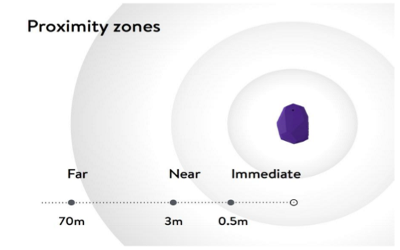
\includegraphics[width=\linewidth]{BeaconsRange}
	\caption{Ejemplificación del rango de un beacon}
	\label{fig:beaconRange}
\end{figure}

Sin embargo, esto depende de como esté diseñada la aplicación, es posible lanzar acciones a una distancia determinada sin tener en cuenta estos rangos mencionados anteriormente, ya que en todo momento es posible conocer la distancia a la que nos encontramos del beacon.

\subsubsection{¿Con qué dispositivos funcionan?}

Las beacons son compatibles con todos los dispositivos que soporten el protocolo Bluetooth Low Energy, pero para que las señales de los beacons sean detectadas por un dispositivo, se ha de tener activado el Bluetooth. 


En dispositivos con IOS7 \cite{URL::IOS7} o superior, el dispositivo puede estar constantemente buscando dispositivos BLE y activar a las aplicaciones implicadas cuando entran en el rango de los beacons, incluso estando cerradas las aplicaciones.


En dispositivos Android \cite{URL::Android} el sistema operativo no está preparado para escanear dispositivos BLE, por lo que son las aplicaciones las que se tienen que encargar de escanear las proximidades buscando beacons, esto supone que las aplicaciones tienen que estar funcionando y despiertas (aunque sea en segundo plano). Existen librerías que solucionan esta limitación, haciendo que la aplicación escanee cada cierto tiempo incluso en segundo plano o estando en ahorro de energía, pero no es muy eficaz y suele tener incompatibilidades ya que induce conflictos con el sistema operativo. Un ejemplo de estas incompatibilidades lo podemos ver en este hilo de discusión \cite{URL::Incompatibilidades} de los desarrolladores de la librería AltBeacon, librería que se ha usado para \BulletPoint{} y que mencionaremos más tarde.

Por último en dispositivos Windows Phone \cite{URL:WindowsPhone} o Blackberry \cite{URL:Blackberry} existen diferentes niveles de compatibilidad pero en los que soportan BLE, su funcionamiento es similar al de los dispositivos Android, por lo que no nos pararemos a analizarlo. 

\subsubsection{¿Qué ventajas y desventajas tienen con respecto a otras tecnologías?}

A la hora de hablar de los beacons existen una serie de ventajas pero también podemos encontrar algunas desventajas que revisaremos a continuación. 

Las principales ventajas que se distinguen a la hora de hablar de los beacons son las siguientes: 

\begin{itemize}
\item A diferencia de la tecnología GPS, la activación del bluetooth consume mucha menos batería. 
\item Las aplicaciones desarrolladas suelen ser dependientes de la red de datos al necesitar información. 
\item A diferencia de la tecnología GPS, sigue funcionando con precisión en el interior de los edificios.
\end{itemize}

En cuanto a las desventajes, podemos destacar las siguientes:

\begin{itemize}
\item Dependen de aplicaciones instaladas en el dispositivo móvil para funcionar. 
\item Es necesario tener el bluetooth activado, lo que consume batería durante el tiempo que esté activado. 
\item Su utilidad depende de la voluntad de terceros de utilizar estos dispositivos, configurarlos y distribuir las aplicaciones.
\end{itemize}

\subsubsection{¿Qué usos se le ha dado a esta tecnología hasta ahora?}

Por ahora esta tecnología se ha utilizado en entornos muy diversos y con distintas funcionalidades. Entre los más conocidos podríamos destacar los siguientes: 

\vspace{5mm}

\textsl{\textbf{{Clevedon School}}}

\vspace{2mm}

Este ejemplo es bastante significativo para nosotros ya que se aplicó en el mismo entorno en el que queremos trabajar, una institución de enseñanza universitaria. Después de desplegar cerca de 1200 iPads  la universidad de Clevedon (Figura \ref{fig:clevedonApp}) utilizó esta tecnología junto con su aplicación universitaria ya existente. 

\begin{figure}[H]
	\centering
	
\includegraphics[width=\linewidth]{ClevedonApp}
	\caption{La aplicación de Clevedon School}
	\label{fig:clevedonApp}
\end{figure}


Han sido capaces de crear una manera fácil para que los profesores puedan añadir recursos que se envían automáticamente a los alumnos transitando diferentes zonas en diferentes horarios. Para realizar este trabajo de manera eficiente fue necesaria la creación de una interfaz para la gestión de los recursos en las diferentes beacons.


Esta interfaz junto con la aplicación móvil es capaz de: 

\begin{itemize}
\item Programar los recursos para distribuirse a una hora del día especificada. 
\item Programar el material para ser distribuido en un momento determinado durante una clase o evento. 
\item Poner los recursos a disposición del alumnado que se encuentre en una localización específica.
\end{itemize}

Utilizando estos tres recursos, la aplicación, la interfaz y los beacons han sido capaces de crear un entorno interactivo y eficiente motivando tanto al profesorado como al alumnado. 

\vspace{5mm}

\textsl{\textbf{{Cleveland Cavaliers Stadium y Levi's Stadium}}}

\vspace{2mm}

Dos de los ejemplos más conocidos han sido los despliegues que se han realizado en estos dos estadios (Ver Figura \ref{fig:levisStadium}). 

\begin{figure}[H]
	\centering
	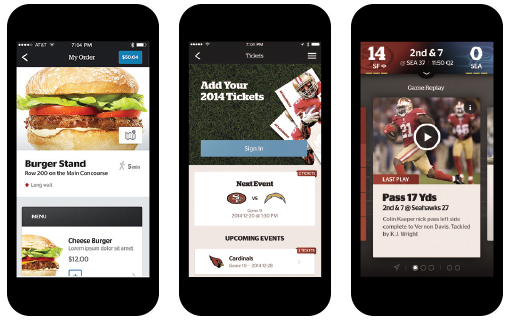
\includegraphics[width=0.8\linewidth]{LevisStadium}
	\caption{La aplicación de Levi's Stadium}
	\label{fig:levisStadium}
\end{figure}

Por un lado tenemos el despliegue del estadio de Levi's , cuya intención ha sido la de ayudar a sus seguidores a navegar por el estadio dadas sus dimensiones. En este caso los beacons (de la comañía Aruba Networks) se utilizan en conjunto con puntos de acceso y repetidores situados por toda la infraestructura de manera que queda el estadio cubierto. Con la aplicación los fanes también son capaces de ver repeticiones de las jugadas y pedir comida directamente desde sus dispositivos móviles.


Un punto importante de este  despliegue ha sido la monitorización continua del funcionamiento de los beacons, incluyendo si están en funcionamiento o necesitan batería nueva. Los beacons son también más económicos que los puntos de acceso WiFi, lo cual les ha beneficiado.

En el caso del estadio de Cleveland, los beacons se encargan de proveer al usuario de información personalizada dependiendo del lugar y la hora. En algunos casos vídeos, ofertas promocionales y contenido adicional.

\vspace{5mm}

\textsl{\textbf{{Orlando Int'l Airport}}}

\vspace{2mm}

Otro despliegue exitoso de esta tecnología ha sido en el aeropuerto internacional de Orlando, donde mediante el uso de los beacons y de una aplicación móvil propia han sido capaces de proporcionar una serie de funcionalidades de vital importancia en una infraestructura como el aeropuerto: 

\begin{itemize}
\item Navegación paso por paso a través de cerca de 1000 establecimientos o servicios dentro del aeropuerto. 
\item Actualizaciones inmediatas de la información de los vuelos. 
\item Intrucciones a puntos de interés criticos como puntos de recogida de equipaje, puertas de embarque o puestos de información.
\end{itemize}

\begin{figure}[H]
	\centering
	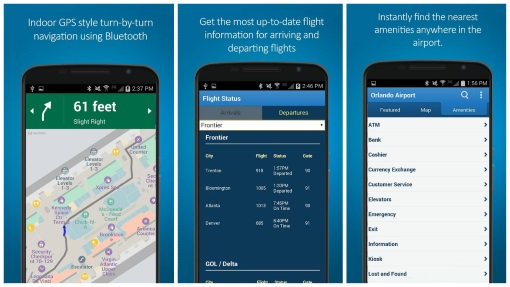
\includegraphics[width=\linewidth]{orlandoAirport}
	\caption{La aplicación del Aeropuerto Internacional de Orlando}
	\label{fig:orlandoAirport}
\end{figure}

El siguiente punto sería ampliar la opción a los establecimientos de ofrecer anuncios o promociones, opción que mantienen abierta y no se descarta en un futuro.


Esta información ha sido extraída de: \cite{URL::Articulo} 

\subsection{CouchBase Server}

Couchbase Server \ref{URL::couchBase} es una base de datos NoSQL \ref{URL::nosql} con una arquitectura distribuida orientada al rendimiento, escalabilidad y disponibilidad. Permite desarrollar aplicaciones de manera sencilla y rápida combinando la flexibilidad del JSON \ref{URL::json} y la tecnología NoSQL.

\subsubsection{¿Por qué utilizar Couchbase Server?}

Hemos decidido utilizar esta tecnología por su flexibilidad y potencia para almacenar documentos fácilmente. Además resulta muy sencillo integrarla con la tecnología móvil mediante el uso de una base de datos reducida dentro del dispositivo móvil (véase Figura \ref{fig:couchbaseexplanation}) sincronizándola con la base de datos principal del servidor mediante una puerta de sincronización.

\begin{figure}[H]
	\centering
	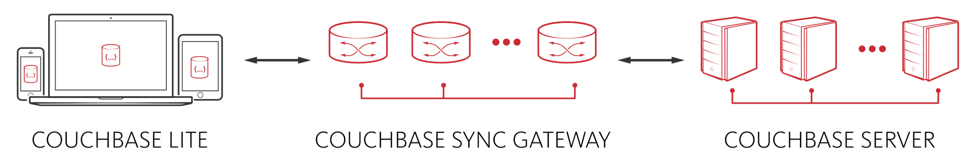
\includegraphics[width=\linewidth]{couchbaseexplanation}
	\caption{Sincronización de CouchBase Server con CouchBase Lite mediante Sync Gateway}
	\label{fig:couchbaseexplanation}
\end{figure}

En este caso se ha configurado el servidor en un ordenador portátil haciendo uso de las indicaciones de la página web del producto \ref{URL::couchweb}. Se procederá a desglosar brevemente los pasos seguidos a la hora de configurar el servidor.


\subsubsection{Configuración de la arquitectura}

Para configurar el servidor se han seguido los siguientes pasos: 


\begin{itemize}
\item Descargar la versión Community del producto desde la página web siguiendo el enlace: \cite{URL::couchbaseDownload}. 
\item Seguir los pasos de la página de desarrolladores para la instalación y configuración: \cite{URL::couchBaseGuide}. 
\item Una vez configurado CouchBase Server procederemos a descargar Sync Gateway que será el servicio que se encargue de sincronizar el contenido del nuestra aplicación al servidor, para ello lo descargaremos de la página al igual que el servidor siguiendo el enlace: \cite{URL::couchbaseDownload} .
\item Para vincular el servidor con Sync Gateway es necesario hacer uso de un fichero de configuración con el que lanzaremos el servicio Sync Gateway.
\item Una vez configurado Sync Gateway, ya tenemos el canal de configuración entre el servidor y la aplicación, para utilizar la base de datos móvil seguiremos los pasos desglosados en: \cite{URL::couchBaseLite} .
\end{itemize}


En este caso se ha tenido que conectar el dispositivo al ordenador. Tanto el ordenador como el dispositivo móvil han de estar en la misma red y hemos utilizado la dirección IP de la máquina para realizar las peticiones del móvil al servidor (alojado en el portátil) al utilizar la API. De esta manera se ha comprobado el funcionamiento del servidor, del servicio de sincronización y de la base de datos versión Lite en el dispositivo móvil.


\subsection{La librería AltBeacon}


\subsubsection{¿Qué es AltBeacon?}

Se puede definir AltBeacon como una especificación que: 

\begin{itemize}
\item Define el formato del protocolo publicitario que los beacons transmiten a través de Bluetooth Low Energy (BLE).
\item Intenta crear un mercado abierto y competitivo para implementaciones usando proximidad con los beacons.
\item Puede ser utilizada gratuitamente, sin cuotas ni compromisos.
\item No favorece a ningún proveedor sobre otro. Las limitaciones vienen determinadas por los estándares técnicos del proveedor.
\end{itemize}

A continuación se profundizará en el funcionamiento y configuración de la librería AltBeacon, que cumple con la especificación AltBeacon y que se ha utilizado para trabajar en Android.

\subsubsection{Configuración}

Para trabajar con esta librería en Android Studio solo hemos tenido que importarla mediante el uso de Gradle a nuestro proyecto como se explica en \cite{URL::importGradle}.


También es posible descargarla desde la página oficial, donde además podremos econtrar diferentes versiones de la misma. Para ello podemos hacer uso del siguiente enlace \cite{URL::versionAltBeacon} y seleccionar la versión deseada.


\subsubsection{Funcionamiento}

La funcionalidad de esta librería se centra en dos elementos principales: 

\begin{itemize}
\item Monitorización (\textit{''Monitoring''}) que sería algo como supervisar, saber qué beacons se encuentran en una región o si ha entrado o salido un beacon de una región.
\item Rastreo (\textit{''Ranging''}), que permite saber a que distancia se encuentran los beacons en todo momento dentro de una región.
\end{itemize}

Utilizando estas dos funcionalidades la aplicación es capaz de controlar, monitorizando y rastreando los distintos beacons en una determinada región. En la página web de la librería \cite{URL::altbeaconSamples} se pueden encontrar ejemplos básicos de como se realizan estas dos funciones en la sección \textit{''Samples''}, además en la sección \textit{''Documentación''} se pueden encontrar también algunos artículos, que pueden resultar interesantes dependiendo del tipo de aplicación que se esté desarrollando.


\subsection{El algoritmo de trilateración}


Durante el desarrollo de este trabajo nombraremos en diferentes puntos el término trilateración. A continuación explicaremos qué es la trilateración y como se ha aplica el algoritmo cuando se trabaja con beacons.

\subsubsection{¿Qué es la trilateración?}


La trilateración es un método matemático para determinar las posiciones relativas de objetos utilizando la geometría de triángulos de forma análoga a la triangulación. La triangulación (utilizada en la tecnología GPS), utiliza medidas de ángulo junto con al menos una distancia para calcular la posición del sujeto. 


A diferencia de esta, y muchas veces confundida con ella por la similitud del término, como podemos apreciar en la Figura \ref{fig:trilateration} la trilateración utiliza las localizaciones conocidas de dos o más puntos de referencia y la distancia medida entre el sujeto y cada punto de referencia. Para determinar de forma única y precisa la localización relativa de un punto en un plano bidimensional usando solo la trilateración se necesitan generalmente al menos 3 puntos de referencia.

\begin{figure}[H]
	\centering
	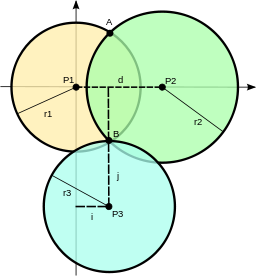
\includegraphics[width=0.6\linewidth]{trilateration}
	\caption{En el algoritmo de trilateración se utilizan las localizaciones conocidas de varios puntos de referencia y la distancia medida entre el sujeto y cada punto de referencia.}
	\label{fig:trilateration}
\end{figure}


En el desarrollo de la aplicación se ha utilizado un algoritmo de trilateración implementado en Java que utiliza el algoritmo de Levenberg-Marquardt \ref{URL::algoritmolm} de Apache Commons Math \ref{URL::apachemath} como explica el autor en \ref{URL::trilateration}. 


En nuestro caso las posiciones de los beacons son determinadas en una imagen separados entre sí a menos de 60 metros. Los beacons se posicionan en esas posiciones elegidas en la imagen y se obtienen posiciones X e Y para cada beacon que quedan registradas en la aplicación (Listado \ref{code:trilaterate}). Las distancias medidas hasta la posición del beacon vienen dadas por la distancia que registra la aplicación a los diferentes beacons. Aparte de estos dos datos para obtener una posición X e Y donde representar el punto es necesario aplicar una escala para convertir los metros a pixeles y obtener el resultado de la posición del usuario en la imagen como una posición X e Y en pixeles.

\lstinputlisting[float, floatplacement=H,caption={Usamos el algoritmo de trilateración, pasándole las posiciones de los beacons y las distancias, el algoritmo los resuelve y devuelve una posición X e Y que transformamos en un objeto de la clase \textit{Point} }, label={code:trilaterate}]
{listings/trilaterateexp.java} %% LISTING

%
% ---------------------------------------------------
%
% Proyecto de Final de Carrera:
% Author: Laura Padrón Jorge <alu0100703511@ull.edu.es>
% Capítulo: Objetivos 
% Fichero: Cap1_Goals.tex
%
% ----------------------------------------------------
%


\chapter{Beacons en entornos universitarios} \label{chap:BeaconsEntornosUniversitarios}  


En este capítulo realizaremos un análisis de los posibles casos de uso de la tecnología beacon en el ámbito universitario.

 
\section{Aplicaciones móviles en entornos universitarios}


Actualmente las posibilidades de las aplicaciones móviles para entornos universitarios se presentan amplias.  Cada universidad intenta tener su propia aplicación siguiendo un patrón similar, puesto que todas parten de necesidades similares. Realizando una investigación general de las aplicaciones disponibles en el mercado observamos que estas aplicaciones se centran en ofrecer servicios propios (servicio de correo, moodle, chat entre usuarios, etc.), mantener al alumnado informado y agilizarle los trámites mayoritariamente. 

En un principio, estas aplicaciones se enfocaban a atraer estudiantes, centrándose en la calidad de la universidad y mostrando las posibilidades que ofrecían. Sin embargo, con el paso de los años y el desarrollo creciente de las aplicaciones móviles, se muestra un cambio en esta estrategia. Ahora las aplicaciones tienen una doble función y no sólo buscan el acceso de nuevos estudiantes, sino que también intentan mejorar la experiencia del alumnado ya matriculado y acercar a los nuevos a la experiencia de la universidad. 



Algunos ejemplos posibles los encontramos en el marketplace de google:

\begin{itemize}
\item \cite{URL::galileo}
\item \cite{URL::valladolid}
\item \cite{URL::oviedo}
\end{itemize}


Uno de los hechos que podemos observar es que las universidades están intentando obtener una solución rápida para desarrollar su app. Una de estas soluciones es la creación de plantillas web optimizadas de su sitio web, lo que podemos considerar una opción rápida con un coste bajo.


Hoy en día casi todos los estudiantes tienen acceso a un dispositivo móvil y cuentan con una tarifa de internet. En un futuro próximo con la aparición de estos dispositivos ya nos surge la pregunta ¿Serán capaces estos dispositivos de transformar la educación? y en caso afirmativo ¿De qué manera? 

\section {Posibles casos de uso de la tecnología beacon en entornos universitarios}

Como se mencionaba antes, una de las posibilidades que se presentan para explotar esta tecnología se encuentra en las instituciones de enseñanza, las cuales podrían utilizar los beacons para facilitar a su alumnado, profesorado y demás personal involucrado  una serie de servicios de gran utilidad.


Sin embargo, para utilizar esta tecnología es necesario cumplir una serie de condiciones:

\begin{itemize}
\item Tener instalada la aplicación en su dispositivo móvil.
\item Tener activado el protocolo bluetooth.
\item La aplicación ha de estar "`activa"'.
\item Los beacons han de estar desplegados y configurados correctamente en lugares clave donde el rango sea óptimo.
\end{itemize}

En el caso de dispositivos Apple no es necesario tener activado el bluetooth ya que el SO se encarga de captar las señales BLE. Tampoco es necesario que la app esté despierta ya que nuevamente el SO se encarga de despertar a la aplicación involucrada. Sin embargo Apple no ha desarrollado un IBeacon físico aún, aunque en un futuro, se espera que sus dispositivos móviles puedan funcionar como un beacon bidireccional. Cabe destacar que existen librerías que se encargan de realizar estas mismas funcionalidades para mantener el móvil despierto a la escucha de posibles beacon para otros sistemas operativos, pero a diferencia de Apple esta funcionalidad no está integrada directamente en el SO por lo que no presenta el mismo nivel de control.


Asimismo, podemos afirmar que prácticamente la mayoría de las universidades cuentan con una disposición amplia en lo que se refiere a servicios y despliegue de medios. Como ejemplo, podemos tomar la Universidad de la Laguna, la cual cuenta con una red WiFi con un rango de cobertura casi completo en sus instalaciones y una amplia carta de servicios disponibles para sus alumnos. Además cuenta con una serie de beacons, que podrían ser instalados fácilmente en lugares estratégicos. 

Partiendo de esta base, procederemos a explorar posibles casos de uso para los beacons tomando el contexto universitario y del alumnado como referente:

\subsection{Guía a través del campus de la universidad}

Este caso de uso cubre la funcionalidad principal de un beacon. El posicionamiento y guía tanto en exteriores como en interiores. 

Como interesados podríamos destacar: 

\begin{itemize}
\item Personal invitado a jornadas o eventos en instalaciones de la universidad.
\item Alumnado de intercambio en programas internacionales.
\item Estudiantes de nuevo acceso.
\item Personas con discapacidad.
\end{itemize}

\begin{figure}[h]
	\centering
	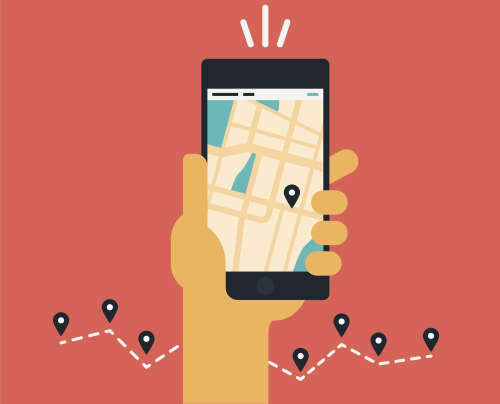
\includegraphics[width=\columnwidth]{locationMobileBeacon}
	\caption{Servicios de localización a través de la Universidad}
	\label{fig:beaconLocation}
\end{figure}

El funcionamiento sería el siguiente: el usuario transita por las inmediaciones del campus universitario. El usuario accede al sistema de navegación dentro de la aplicación, la cual le muestra entonces el indocándole  en todo momento su ubicación como un punto de color sobre el mapa del campus. Este mapa tiene marcados puntos de interés que contienen información de diferente tipo dependiendo del punto marcado: nombre, historia, página web, teléfono de contacto, trámites asociados... son algunos de los datos que podría mostrar. El mapa se va actualizando dependiendo de la posición del usuario permitiendo volver a la vista más alejada en cualquier momento para una visualización más general.


\subsection{Descarga automática de material} \label{sec:descargaautomatica}

Este caso de uso resultaría muy útil para personal lectivo y para estudiantes, los cuales accederían de manera más sencilla al material disponible. También sería aplicable para ponentes de charlas quienes no tendrían que alojar sus apuntes en alguna plataforma externa o llevarlos consigo en  un almacenamiento externo para compartirlo al finalizar la actividad.

El funcionamiento sería el siguiente: el profesor/a o ponente lleva consigo un beacon y sus estudiantes u oyentes tienen instalados en sus dispositivos la aplicación. El profesor es capaz de introducir en su aplicación con el perfil de profesor (el ponente con su correspondiente perfil), indicaciones del material a utilizar en el evento. El profesor/a carga consigo el pequeño dispositivo e indica al alumnado que conecten el bluetooth y abran la aplicación. Al entrar en el rango, la app pedirá permiso al alumno para descargarse el contenido indicado por el profesor. Si el alumno acepta, la aplicación pasaría a abrir  el contenido indicado por la página correspondiente.


\subsection{Acceso al parking y recuento de número de plazas disponibles}


Este caso de uso proporcionaría información muy útil a los usuarios del parking de la universidad, informando del número coches estacionados en el parking y de las plazas restantes a ocupar en tiempo real.

El funcionamiento sería el siguiente: el personal de la ULL tendría la aplicación en su móvil; al acercarse a la barrera del parking, el usuario activaría el bluetooth de su móvil. La app registraría un nuevo punto entrando en el rango de acción del parking. La aplicación comprobaría conectando con un servidor institucional que el usuario está autorizado a entrar en el parking y procedería a abrir la puerta del parking dejando entrar al vehículo. Cuando el vehículo saliese del rango del beacon por el rango interior, la aplicación registraría entonces un nuevo acceso al parking y contabilizaría otro vehículo dentro de parking. Al salir del parking el proceso sería el mismo, por lo tanto la aplicación sería capaz de informar al usuario de las plazas ocupadas en tiempo real.


\subsection{Gestión de eventos e información, entrada automática}

El funcionamiento sería el siguiente: el alumnado transita los interiores de la Universidad de camino a sus clases. Los beacons están desplegados en las inmediaciones de lugares de interés, tipo aulario, paraninfo, clases que se utilicen a modo de salas de reuniones o seminarios. Al pasar por las inmediaciones de estos lugares de interés, la aplicación sería capaz de proporcionar al usuario información de diversa índole: ponentes, tema de la charla, acceso, teléfono de contacto u otra información similar.  Al mismo tiempo, la aplicación también cuenta con un tablón donde se muestran posibles eventos futuros. Estos eventos pueden ser muy variados y corresponder a diferentes tipos de actividades. Al mismo tiempo se podría confirmar la entrada al evento en el caso de haberla, mediante un código de acceso identificativo generado al realizar la inscripción en el evento.

\begin{figure}[H]
	\centering
	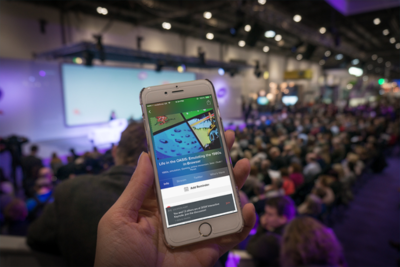
\includegraphics[width=\columnwidth]{BeaconEvent}
	\label{fig:eventBeacon}
\end{figure}

\subsection{Despacho del profesorado e información}

El funcionamiento podría abarcarse de dos maneras. Por un lado, podría utilizarse para proveer al alumnado de información acerca del grupo de despachos, aclarando que profesorado tiene el despacho en la zona, horario de tutorías, correo electrónico de contacto, horario de corrección de exámenes, etc. De esta manera el alumnado al acercarse a la zona sería capaz de acceder a información de todo el profesorado, o si buscase a alguno en particular, la aplicación le daría la opción de elegir su nombre de una lista y simplemente comprobar si tiene su despacho en esa zona. 

Por otro lado, este caso de uso podría ampliarse para proporcionar una información adicional, comprobando si el profesorado está en la zona en ese momento y se encuentra disponible. El profesor tendrá un perfil de la aplicación con un código identificativo que le distingue de los demás profesores. Estos datos se guardarían en un servicio externo, y la app sería la encargadada acceder a este servicio consultando las entradas y salidas del profesorado. De esta manera el alumnado sería capaz de saber cuando el profesor se encuentra disponible en las cercanías mediante la aplicación. En cuanto al estado de disponibilidad, sería un dato que actualizaría el profesor desde su perfil en la aplicación. 

\subsection{Información y descuentos para usuarios de la app}

Este caso de uso no solo dependería de la universidad, sino de establecimientos comerciales interesados. La idea sería la siguiente: la universidad en colaboración con un establecimiento comercial le entrega un beacon. La aplicación contaría con un perfil para el dueño del establecimiento, donde sería capaz de introducir información que desea que se muestre al usuario al pasar cerca de su establecimiento, mensajes de información, descuentos u ofertas especiales por ejemplo. 

El usuario al pasar por las inmediaciones del establecimeinto recibe en su aplicación una notificación del establecimiento con la información introducida por el dueño anteriormente. Al aceptar la notificación, el usuario podría ser redirigido a la página web del establecimiento para ver las ofertas. En cualquier caso el establecimiento ha conseguido captar la atención de un posible cliente, y el usuario se benefiaría de ofertas y descuentos. 

\subsection{Control de asistencia}

Este caso de uso podría ir ligado al de descarga automática de material (véase epígrafe \ref{sec:descargaautomatica}), el funcionamiento sería el siguiente: el alumno conectaría el bluetooth de su móvil al iniciar la clase. En este momento la aplicación detectaría los dispositivos con los identificadores de DAS del alumnado y los dejaría registrados a la clase en el horario establecido. El profesorado sería capaz en todo momento desde el perfil de profesor de consultar la asistencia. Si lo unimos con la descarga automática de material, proporcionaría comodidad tanto al alumnado como al profesorado. Sin embargo, un impedimento podría ser el rango del beacon o la necesidad de activar el bluetooth ya que, si el alumno no tiene batería en el móvil, tendría que haber un método secundario. 

\subsection{Control de acceso a instalaciones}

En control de acceso a las aulas y edificios puede ser un tema abordable mediante el uso de estos dispositivos. Los lectores de tarjetas pasarían a ser algo innecesario. El alumno simplemente tendría que activar el bluetooth cerca del punto de acceso, se comprobaría su identidad y procedería a darle a acceso o a informarle de su falta de permiso para acceder. Los permisos de acceso a estos puntos podrían quedar almacenados en algún tipo de plataforma donde se monitorizen los accesos dependiendo de la seguridad de acceso al aula.

\subsection{Biblioteca informativa}

Otro posible uso que se le podría dar a la tecnología beacon tiene que ver con las bibliotecas o lugares de almacenamiento de material. El estudiante se acercaría a la biblioteca buscando un libro específico, en la aplicación estaría registrada la localización de los libros disponibles en los estantes, lo que le indicaría al alumno/a la posición del libro que busca. Para lugares amplios donde hay gran cantidad de material (véase la Figura \ref{fig:bibliotecaUSAL}), incluso podría guiar al usuario como un punto por las instalaciones hasta llegar a su objetivo, informarle de si quedan ejemplares disponibles o de la fecha prevista de entrada de algún material, de esta manera el alumnado agilizaría su búsqueda en gran medida.

\begin{figure}[H]
	\centering
	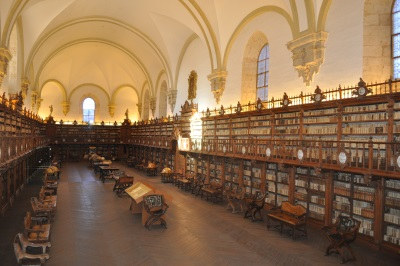
\includegraphics[width=\columnwidth]{BibliotecaSalamanca}
	\caption{La biblioteca de la Universidad de Salamanca contiene más de 1.000.000 de ejemplares lo que puede dificultar la localización de algunos títulos.}
	\label{fig:bibliotecaUSAL}
\end{figure}

\subsection{Actividades interactivas por el campus, jornadas de acogida u otros eventos}

En un ámbito más recreativo, se podría tener en cuenta el uso de los beacons para organizar juegos o actividades de ocio para el alumnado. Estos eventos dependerían de los organizadores, pero podrían consistir en alguna actividad que implicase movimiento y colaboración. El alumnado tendría que registrarse con su identificador. Una ruta a través del campus con adivinanzas o puzzles que tengan que ver con diferentes temáticas por ejemplo fomentaría al alumnado a trabajar en equipo y utilizar su ingenio. Al mismo tiempo se podría aplicar algún tipo de recompensa para los ganadores, descuentos o bonos tramitados por medio de la aplicación, lo que fomentaría la participación estudiantil.

\subsection{Localización de transporte público, horarios e información de la parada}

Uno de los transportes más utilizado por el alumnado de la universidad es el autobús. Este medio de transporte puede llegar a ser el día a día de muchos de los estudiantes que no cuentan con vehículo propio o que simplemente prefieren utilizar este medio de transporte. 

Este caso de uso contempla lo siguiente: El estudiante llega a una parada de autobus y utilizando su dispositivo móvil, consulta los autobuses que van a pasar por la parada. La aplicación le permite obtener información de los diferentes autobuses, el itinerario y el tiempo restantes para que llegue a la parada.  Asimismo también enlazaría con la web de la compañía de transporte para más información sobre las líneas y los itinerarios en caso de necesitar más información que la proporcionada por la app.
% ---------------------------------------------------
%
% Trabajo de Fin de Grado. 
% Author: Laura Padrón Jorge. 
% Capítulo: La aplicacion BulletPoint. 
% Fichero: Cap4_TheApplication.tex
%
% ----------------------------------------------------
%

\chapter{La aplicación BulletPoint} \label{chap:LaAplicacion} 

Basándonos en los casos de uso revisados en el capítulo anterior, en este capítulo se discutirán los casos de uso que han sido elegidos e implementados en la aplicación \BulletPoint{}. Comentaremos la aplicación centrándonos en el desarrollo de la misma, así como  en diferentes partes a destacar del código que puedan resultar interesantes.


\section{Casos de uso elegidos}

Como ya hemos mencionado previamente, estos casos de uso se incluyen como parte de la aplicación que se ha desarrollado en este TFG, donde cada caso de uso se considera un módulo. La integración de cada uno de estos módulos con el resto de la aplicación se ha realizado mediante el desarrollo de un menú de funcionalidades donde es posible seleccionar qué acción se desea. Para almacenar la información necesaria para algunos módulos, se ha introducido un menú adicional de ajustes. Estos datos se utilizan entre otras cosas para identificar al usuario y confirmar ciertas acciones o dejar constancia de otras. 


A continuación se desglosarán los distintos casos de uso en los que tendremos que pensar de ahora en adelante como módulos, junto con la explicación del caso de uso y su funcionamiento se incluirán algunos de los detalles más importantes de la implementación de cada uno.

\subsection{Localización de transporte público, horarios e información de la parada}

\subsubsection{Objetivo}


El objetivo de este caso de uso es el conocer, en tiempo real, qué autobuses pasan por la parada en la que nos encontramos, hacia dónde se dirigen, y cuánto tiempo falta para que lleguen a la parada. En caso de necesidad de información adicional, la aplicación está preparada para remitirnos a navegar por la página web \cite{URL::titsa} de la empresa Transportes interurbanos de Tenerife, S.A.(TITSA), donde podemos ver datos adicionales sobre el autobús seleccionado.

\begin{figure}[H]
	\centering
	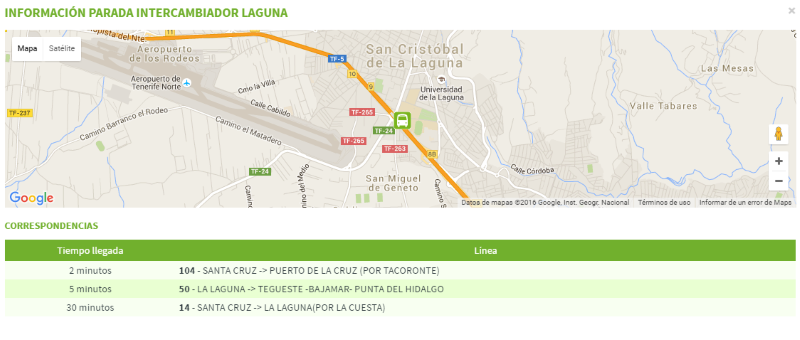
\includegraphics[width=\columnwidth]{titsaMap}
	\caption{La información mostrada por TITSA actualmente en su página web.}
	\label{fig:MapaTitsa}
\end{figure}

\subsubsection{Despliegue}

En este caso, sería necesario colocar un beacon en cada parada de guaguas. De esta manera cada parada de guagua queda identificada por un beacon. Si el usuario se encuentra cercano a dos paradas, la aplicación considera que le interesa la información de la parada más cercana a su posición y le proporcionará información únicamente de esta parada con el objetivo de no confundir al usuario.

\subsubsection{Funcionamiento}


Mediante el uso de los beacons, permitimos a la aplicación identificar en que parada se encuentra el usuario. La aplicación asocia la MAC \ref{el:mac} de un beacon con el número identificativo de la parada. Este número identificativo de la parada es lo que utiliza TITSA para identificar sus paradas en la API y en toda su web. En el listado \ref{code:beaconbusstop}

\vspace{5mm}

\lstinputlisting[caption={\textit{BusBeaconStop}. Esta clase contiene la información que asocia cada MAC con el ID de la parada de TITSA. añadir un nuevo beacon a una parada implicaría añadir un nuevo elemento a \textit{stopsMapId}.}, label={code:beaconbusstop}]
{listings/BeaconBusStop.java} %% LISTING

\vspace{5mm}

La aplicación ha sido programada enlazando los números identificativos de la parada con la dirección MAC de los beacons. Cuando la aplicación detecta un beacon es capaz de reconocer la parada en la que se encuentra el usuario. Una vez la aplicación conoce los datos de la parada, se procede a realizar dos peticiones de comunicación con el servicio de TITSA: 


\begin{itemize}
\item La primera petición se hace sobre la API de TITSA que nos proporciona la información de los autobuses y el tiempo restante para que llegue dicho autobús a la parada. Cabe destacar que para poder utilizar esta API se contactó con TITSA, cuyo personal nos proporcionó una API KEY para poder trabajar con ella. Podemos ver el método principal en el listado \ref{code:basedOnLineNumber}.

\vspace{5mm}
\lstinputlisting[caption={El método \textit{getTimetablesBasedOnLineNumber()} del cliente de TITSA se encarga de obtener los datos de su API y devolver una lista de llegadas.}, label={code:basedOnLineNumber}]
{listings/HttpClientTitsa.java} %% LISTING
\vspace{5mm}

\item La segunda petición se realiza sobre la web de TITSA directamente. El objetivo de esta petición es obtener para cada autobús la información de su recorrido. Para ello se obtiene el código de la página en HTML extrayendo la información relativa a su itinerario. La información no se encuentra en un formato óptimo en algunos casos, pero esta información proviene de TITSA y ofrece una información necesaria para usuario. 
\end{itemize}

\lstinputlisting[float, floatplacement=H, caption={La clase \textit{Arrival} donde quedan contenidos los datos de cada llegada.}, label={code:arrival}]
{listings/Arrival.java} %% LISTING

Aparte de esta información por cada autobús se incluye un enlace a modo de botón, que redireciona al usuario a la página web de TITSA con el identificador de la línea, con lo que el usuario puede obtener más información adicional en caso de precisarla.


En un principio, nuestra idea era utilizar simplemente la API de TITSA, puesto que se creía que proporcionaría toda esta información, sin embargo en algunos casos, los destinos no se correspondían con la realidad, y las rutas aparecían erróneas. Ante esta situación, se contactó con personal de  TITSA involucrado en el desarrollo de esta API quien nos comentó que esto ocurría en algunos casos por la manera en la que estaba planteada la API.


La solución que se adoptí, fue utilizar ambos métodos para obtener la información completa. Ambos métodos serán desglosados a continuación: 


En el primer método, utilizando una librería de peticiónes HTTP, se envía una consulta por GET a la API de TITSA que devuelve una respuesta en XML. Esta respuesta se parsea con un handler de XML (véase Listado \ref{code:handler}). 

\lstinputlisting[float, floatplacement=H,caption={El handler se encarga de transformar el fichero XML en elementos de tipo \textit{Arrival} (véase Listado \ref{code:arrival}).}, label={code:handler}]
{listings/XmlHandler.java} %% LISTING

Al mismo tiempo, se inicia la petición a la página de TITSA y utilizando la librería Jsoup \cite{URL::Jsoup}, se obtiene el contenido de la página web. De este contenido en HTML, recopilamos únicamente el recorrido de los autobuses y el resto se descarta como podemos ver en el listado \ref{code:jsoup}. Esta petición es bastante más pesada que la del XML previa, ya que tiene que obtener todo el contenido de la página web en la que aparece el desglose del itinerario en formato HTML. El parseo de la página también es más lento que en el paso previo, ya que tiene que ir elemento por elemento iterando en los elementos hijos del HTML.

\lstinputlisting[float, floatplacement=T,caption={El método \textit{getCorrectRoute()} nos permite obtener el itinerario correcto del autobús.}, label={code:jsoup}]
{listings/HttpClientTitsaJsoup.java} %% LISTING

\begin{figure}[H]
	\centering
	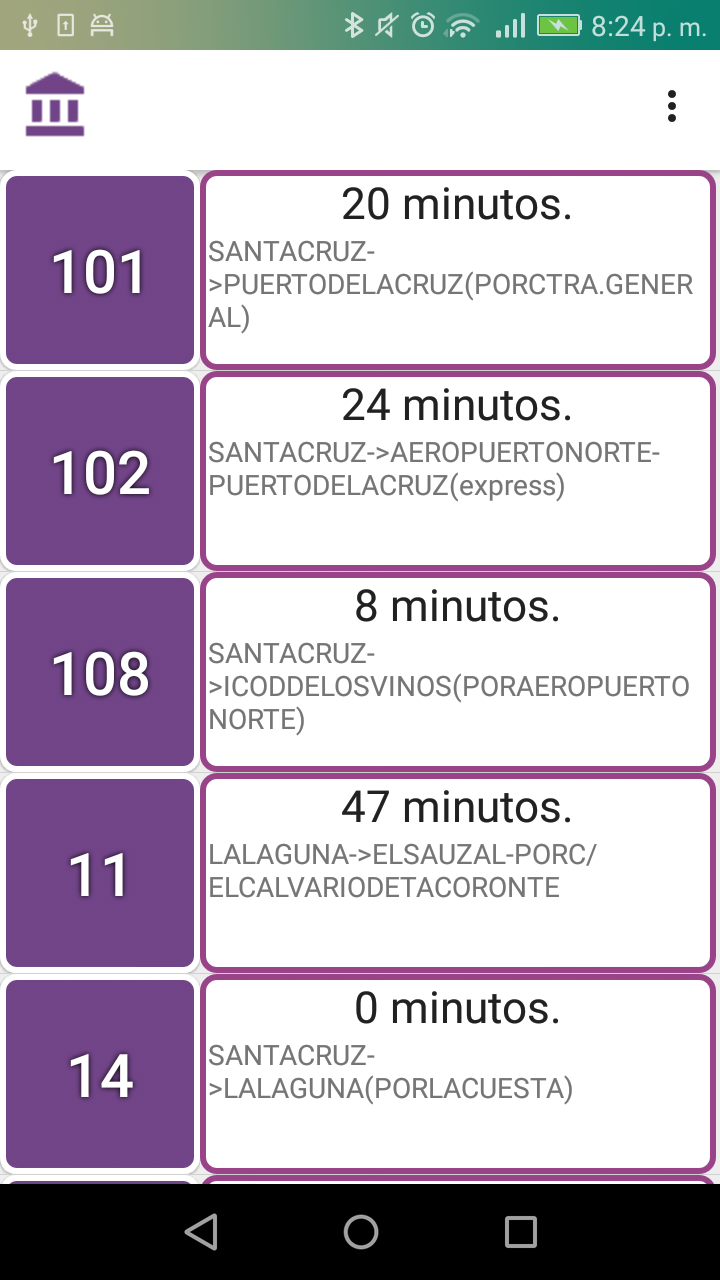
\includegraphics[width=60mm,height=100mm]{Autobuses}
	\caption{\BulletPoint{} permite conocer en tiempo real, autobuses que se acercan a la parada, junto con su destino y tiempo de llegada de la parada identificada por un beacon.}
	\label{fig:autobuses}
\end{figure}

Utilizando ambos conjuntos de datos, se va creando una estructura con los datos, donde se almacena la información sobre cada elemento. En última instancia se van añadiendo estos elementos a la vista utilizando un adaptador y una estructura para visualizar listas.


\subsubsection{Dificultades}


A la hora de plantear este caso de uso se han detectado las siguientes dificultades: 

\begin{itemize}
\item A la hora de presentar los datos, la generación de la estructura era un proceso con el que no se estaba familiarizado y que ha llevado más tiempo del previsto, pero que ha servido de piedra angular para el desarrollo de los demás casos de uso ya que presenta elementos comunes: peticiones, parseo de datos, visualización de listas, etc.
\item Otra dificultad ha sido el no poder obtener todos los datos necesarios con una sola petición y tener que hacer uso de dos peticiones distintas, con el tratamiento posterior de estos datos, ya que no eran en absoluto similares.
\end{itemize}


\subsubsection{Ampliación}

Ampliar este caso de uso sólo conllevaría asociar los nuevos identificadores de los beacons a nuevos identificadores de parada. Por ello podemos afirmar que sería relativamente sencillo desplegar una red de beacons en las paradas de guagua de TITSA en este caso y obtener esta información de manera sencilla. 


\subsection{Gestión de eventos e información}

\subsubsection{Objetivo}

El objetivo de este caso de uso sigue siendo el de proporcionar información de eventos e información de interés para el usuario; sin embargo, se ha desligado el módulo de entrada automática, al que hacíamos mención en el análisis previo, ya que en la mayoría de los casos esta funcionalidad no es necesaria.  


\subsubsection{Despliegue}


En este caso, sería necesario colocar un beacon en sitios de interés donde puedan tener lugar eventos. Al mismo tiempo, también es necesaria una fuente de datos donde alojar la información de los eventos. De esta manera cada beacon referenciaría a una fuente de información de eventos. Si el usuario se encuentra cercano a dos beacons, la aplicación considera que le interesa la información del beacon más cercano a su posición. Si se desplaza a otra posición y se acerca a otro beacon, la información sería diferente.

\subsubsection{Funcionamiento}


Mediante el uso de los beacons, permitimos a la aplicación identificar en qué localización se encuentra el usuario. En este caso, hemos utilizado la información RSS del portal web eventosULL \cite{URL::eventsull}. Esta página posee diferentes enlaces RSS, actualmente no están separados por ubicación sino por categorías variadas (ocio, eventos, deportes, tecnologías,etc.). Sin embargo lo hemos tomado como ejemplo porque constituye un portal que ya está en funcionamiento y proporciona información sobre eventos actuales relacionados con la Universidad de la Laguna. 


La aplicación ha sido programada enlazando la dirección MAC de los beacons con diferentes enlaces RSS de la página web de eventos como podemos apreciar en el listado \ref{code:rss}. Al detectar un beacon, se reconoce a qué información queremos acceder y se procede a realizar una petición utilizando el enlace identificado por el beacon: 

\lstinputlisting[float, floatplacement=H, caption={La información de la MAC del beacon queda asociada a un enlace RSS.}, label={code:rss}]
{listings/RssBeaconInfo.java} %% LISTING

La petición se lanza sobre el enlace, el cual nos devuelve un archivo XML que procedemos a tratar para extraer la información que nos interesa. Para no sobrecargar la aplicación con demasiada información del evento hemos decidido utilizar sólo los datos más relevantes: el título y la fecha del evento. Al mismo tiempo, sobre cada evento se incluye un enlace que al ser seleccionado remite a la página web del evento seleccionado para suministrar información adicional sobre él (localización en un mapa, manera de inscribirse al evento, etc.). Sin embargo, esta información no está disponible para todos los eventos.


En un principio, se planteó el filtrar los eventos para obtener los cercanos a una posición geográfica; sin embargo, no todos los eventos poseen esta información, y sería necesario realizar una petición por cada RSS para obtener los datos con lo que se tardaría mucho más y el proceso sería más lento. Si en el futuro se planteara, cada RSS debería relacionarse con la localización del evento.

\begin{figure}[H]
	\centering
	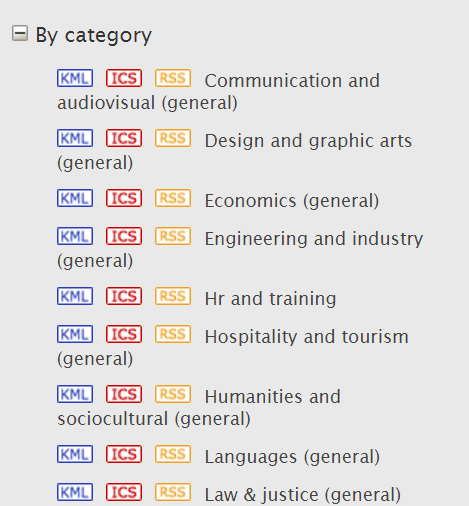
\includegraphics[width=85mm,height=70mm]{eventsRss}
	\caption{Las diferentes categorías de los RSS del portal web de eventos.ull.es}
	\label{fig:eventsRss}
\end{figure}


La petición se realiza utilizando la misma librería de peticiones HTTP que en el caso anterior: se envía una consulta por GET al enlace RSS de la página web de eventosULL el cual nos devuelve una respuesta en XML. Esta respuesta se parsea con un handler de XML para seleccionar únicamente los datos que nos interesan. Esta petición es bastante rápida y genera una vista con la información de los distintos eventos. Cada elemento evento de esta lista es capaz de remitir a la página web de eventosULL para recibir información adicional en caso de estar interesados en el evento en cuestión.

\begin{figure}[H]
	\centering
	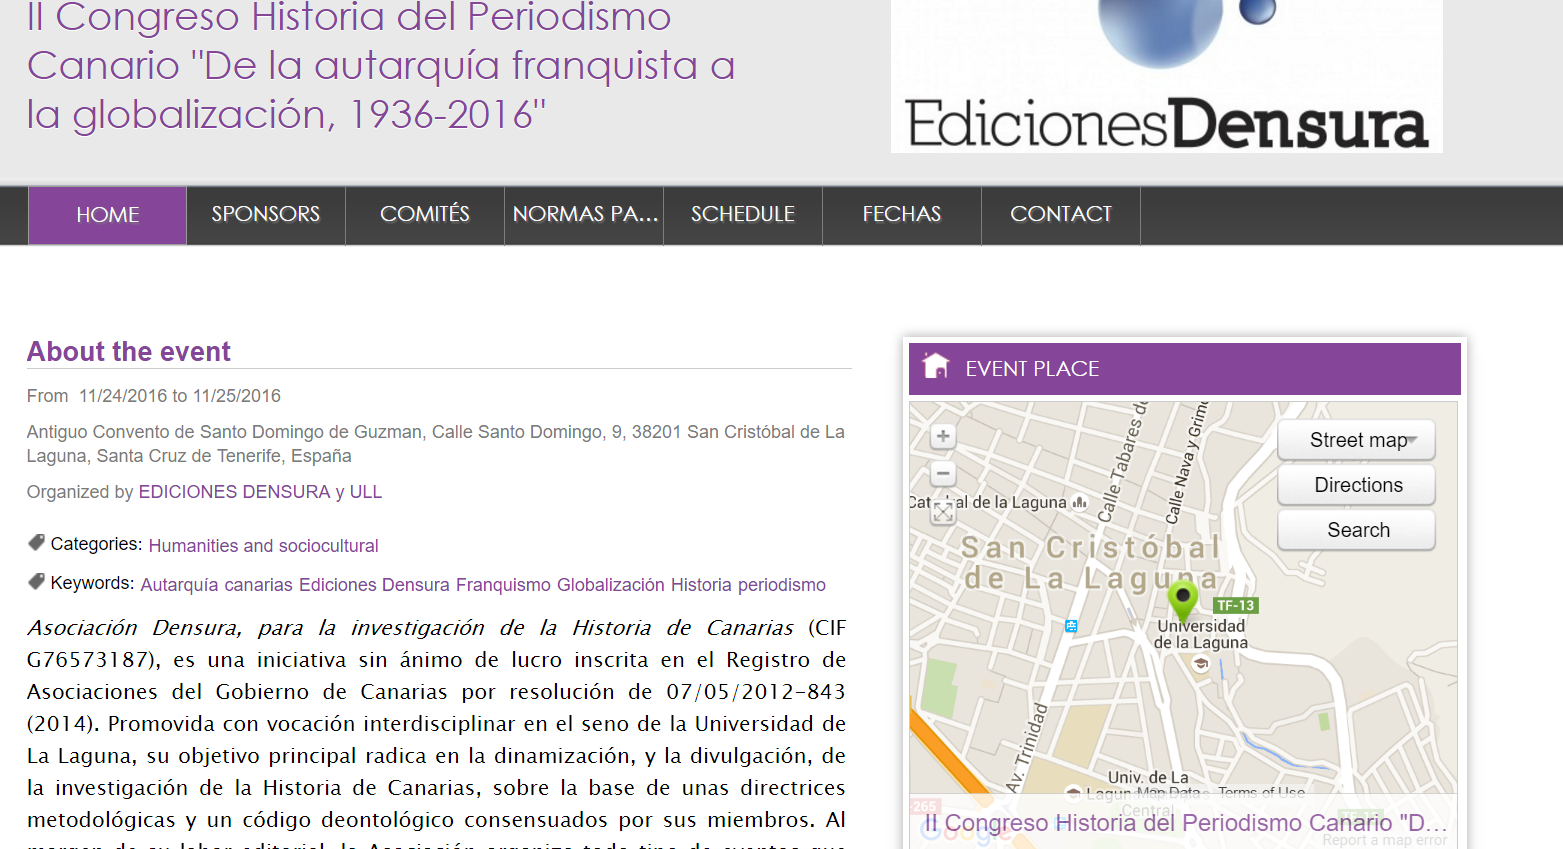
\includegraphics[width=\columnwidth]{eventsPage}
	\caption{El portal web de eventos, donde podemos obtener información adicional de un evento concreto.}
	\label{fig:eventsPage}
\end{figure}

\begin{figure}[H]
	\centering
	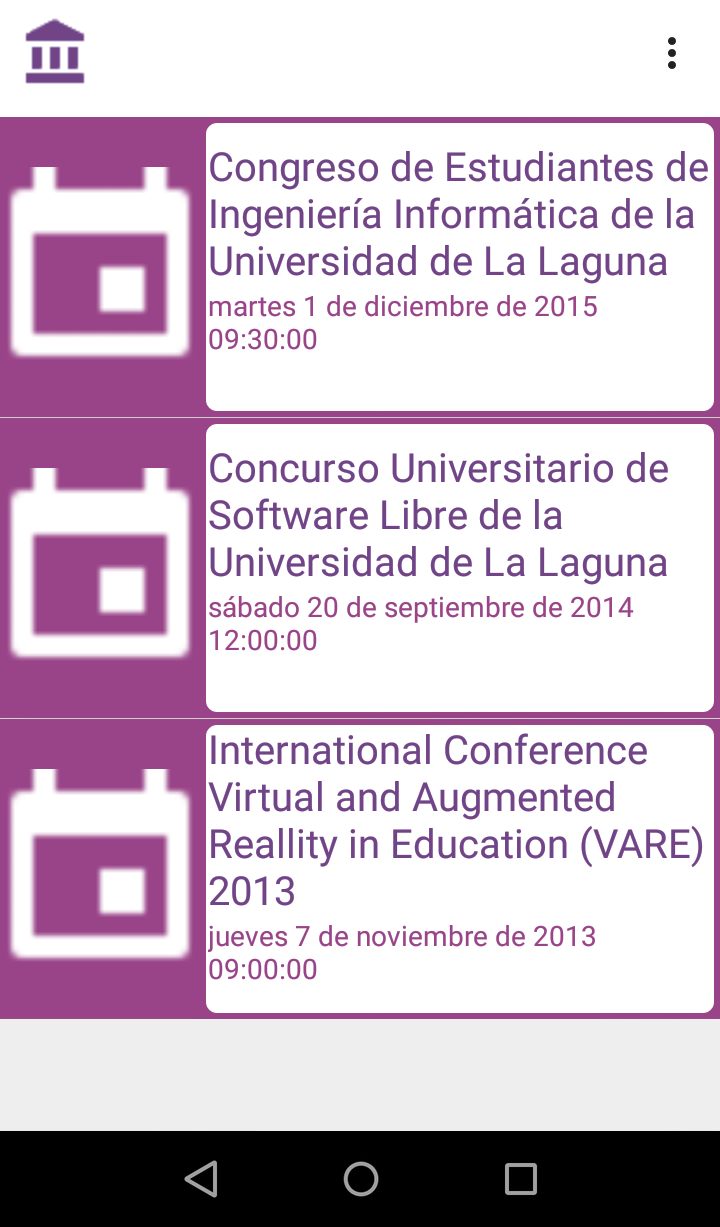
\includegraphics[width=60mm,height=100mm]{Eventos}
	\caption{Podemos conocer eventos asociados a un RSS del portal web.}
	\label{fig:eventos}
\end{figure}

\subsubsection{Dificultades}


A la hora de implementar este caso de uso no ha habido grandes dificultades, si bien la fuente de datos no ha sido la óptima, ya que lo ideal hubiese sido poder filtrar los eventos por localización en lugar de por categorías. Sin embargo, se ha conseguido el objetivo principal de mostrar diferentes eventos en función del beacon detectado.

\subsubsection{Ampliación}


Ampliar este caso de uso sólo conllevaría asociar los nuevos identificadores de los beacons a nuevos identificadores de ficheros RSS. Es por ello que podemos afirmar que sería relativamente sencillo desplegar una red de beacons en diferentes puntos del campus universitario asociados a un RSS. En caso de utilizar otro medio al RSS, sólo habría que adaptar la obtención y la visualización del nuevo contenido, modificando la dirección y añadiendo un nuevo parseo.


\subsection{Control de asistencia}

\subsubsection{Objetivo}

Este caso de uso tiene como objetivo controlar la asistencia de los alumnos a las clases u otro evento que requiera control de asistencia. En un principio se había descartado por las complicaciones que presentaba: 

\begin{itemize}
\item Era necesario tener un servidor en el que poder almacenar la información de las asistencias con la información de los participantes.
\item Se necesitaba un modo de almacenar los datos del usuario para poder identificarle a la hora de registrar la asistencia.
\item El área de acción para registrar la asistencia podía ser variable, sin ser muy exacta. El rango podía salirse del aula o localización de la actividad.
\item Debía haber algún tipo de control para no registrar asistencias erróneas o fraudulentas.
\end{itemize}

Para solucionar estos problemas se ha optado por las siguientes soluciones: 

Como servidor se ha utilizado \textit{``Couchbase Server"}, una base de datos distribuida no-SQL, orientada a documentos y de código abierto. Por otro lado, se ha configurado en la aplicación móvil una base de datos \textit{``Couchbase Lite"} que sirve de paso intermedio e interactúa con \textit{``Sync Gateway"} para sincronizar los datos de la base de datos del dispositivo al servidor, y viceversa.


Para almacenar los datos del usuario se ha hecho uso de la API de preferencias de Android como podemos apreciar en los listados \ref{code:loadpreferences} y \ref{code:xmlpreferences}, el cual almacena los datos en el dispositivo móvil en un espacio compartido para toda la aplicación. De esta manera, se han almacenado datos como \textit{``Nombre de Usuario"}, \textit{``Número Das"} o \textit{``DNI"}, los cuales solo serán visibles para el usuario de la aplicación y servirán para registrar las asistencias con estos datos.

\lstinputlisting[float, floatplacement=H, caption={Para cargar la pantalla de preferencias de un fichero XML en el fragmento \textit{Settings}.},label={code:loadpreferences}]
{listings/SettingsActivity.java} %% LISTING

\vspace{5mm}
\lstinputlisting[language=xml, caption={El fichero XML de donde se cargan todas las preferencias.},label={code:xmlpreferences}]
{listings/preferences.xml} %% LISTING
\vspace{5mm}

En cuanto al área de acción a partir de la cual es posible registrar la asistencia, se ha optado por establecer un perímetro dentro del aula delimitado por las paredes de la misma, descartando cierto margen, de manera que el aula quede cubierta y los exteriores no se tengan en cuenta. 

\subsubsection{Despliegue}

En este caso, para poder realizar este proceso es necesario utilizar la trilateración \cite{URL::trilateracion} por lo que, es necesario desplegar al menos 3 beacons. Para las pruebas se ha utilizado el aula 2.1 del Edificio de Ingeniería Informática. Estos beacons no tienen que ser necesariamente por aula ya cada beacon cubre un área de 70 metros de radio aproximadamente; teniendo en cuenta que las paredes crean interferencias en la señal, probablemente se podrían utilizar 3 beacons para cubrir dos aulas, pero habría que hacer un estudio de la localización y las interferencias para poder asegurarlo. 

\subsubsection{Funcionamiento}


En cuanto se accede al módulo de asistencia, la aplicación comienza a escanear las inmediaciones buscando beacons. Cuando detecta más de 2 beacons, la aplicación carga la imagen de dicha localización y comprueba que el alumno se encuentra dentro de la zona delimitada para registrar la asistencia, listado \ref{code:scanAtt}.

\begin{figure}[H]
	\centering
	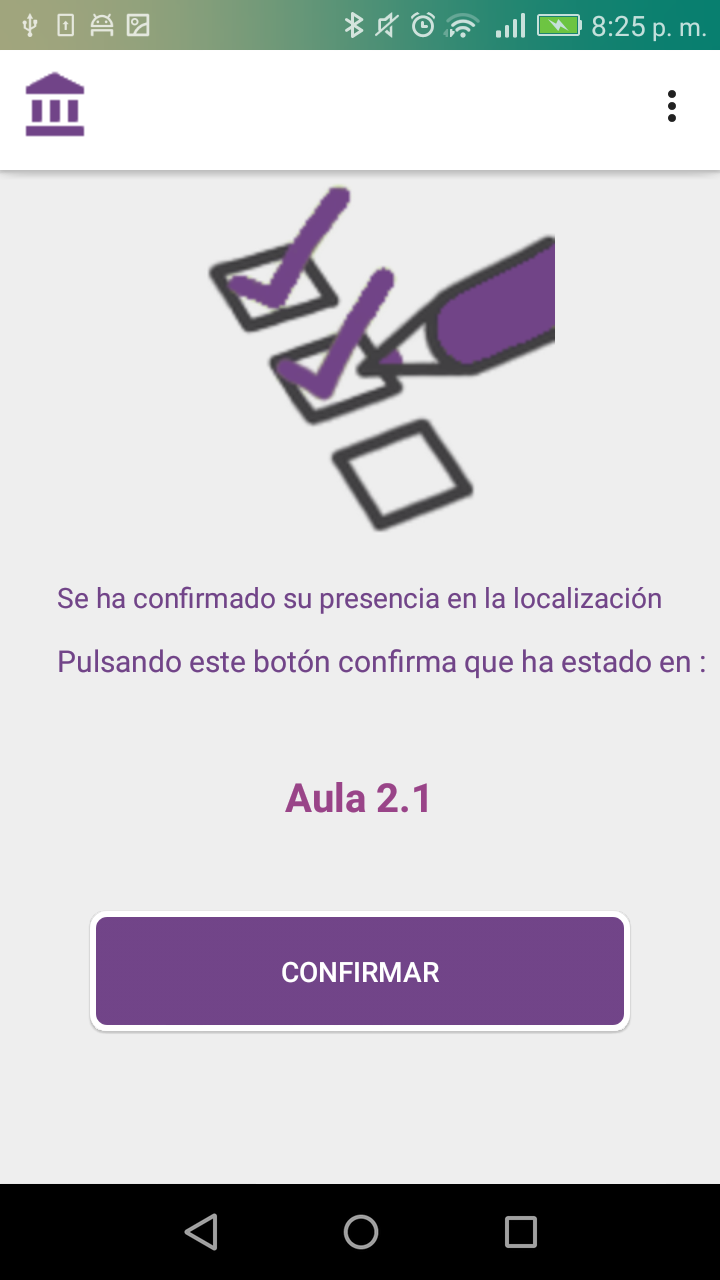
\includegraphics[width=80mm,height=120mm]{ConfirmarAsistencia}
	\caption{Pantalla de confirmación de asistencia en la localización.}
	\label{fig:confirmarAsistencia}
\end{figure}

\lstinputlisting[float, floatplacement=H, caption={Utilizando \textit{ScanFragment} se comprueba que el usuario se encuentra dentro de la zona delimitada.},label={code:scanAtt}]
{listings/scanAtt.java} %% LISTING

Si no se encuentra en la zona delimitada, igualmente la aplicación muestra su ubicación en el mapa para que pueda corregir su posición. Una vez que acceda al área se muestra un mensaje de confirmación con el aula en la que se encuentra. En este momento se debe confirmar (Véase Figura \ref{fig:confirmarAsistencia}) pulsando un botón de que el usuario desea registrar la asistencia. Previamente el usuario ha debido introducir sus datos en la aplicación y éstos deben estar almacenados. Estos datos son los que utiliza la aplicación, junto con la dirección MAC del dispositivo desde el cual se envía la petición de registro. Otro control es almacenar una hora junto con los demás datos, a la hora de enviar la información al servidor, asegurándonos de que realmente el usuario ha estado en el aula a dicha hora.


Los datos que se almacenan en el servidor tienen estructura que se muestra en a Figura \ref{fig:couchDBsctructure}, sin embargo esta estructura puede ser fácilmente modificada si se detecta que es necesario añadir más datos.

\begin{figure}[H]
	\centering
	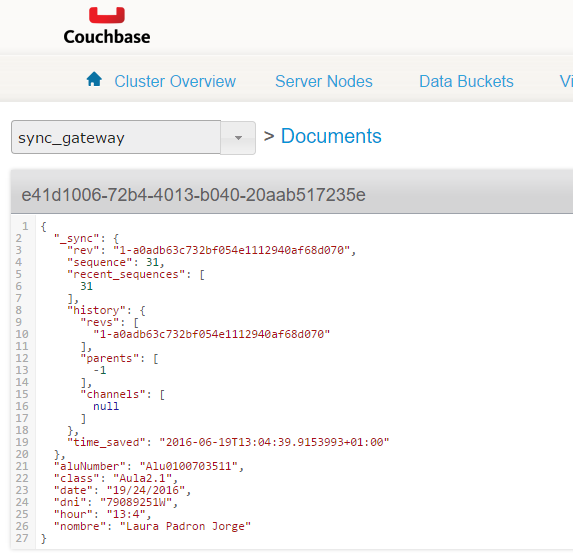
\includegraphics[width=\columnwidth]{couchDBstucture}
	\caption{La estructura de los datos del usuario en CouchBase Server.}
	\label{fig:couchDBstucture}
\end{figure}


\subsubsection{Dificultades}

En este caso las dificultades han sido de diversa índole, se ha tenido que configurar un servidor con el que no se había trabajado previamente, se ha tenido que trabajar con la API de preferencias de Android, y había que idear un método que permitiese comprobar de manera fiable que el alumno se encontraba o había estado en la localización a la hora correcta. La configuración del servidor y Sync Gateway ha sido un poco tediosa, pero una vez configurada es muy fácil de utilizar.


\subsubsection{Ampliación}

Para ampliar este caso de uso se deberían incluir nuevos beacons, nuevas imagenes de las localizaciones y nuevas áreas de registro; sin embargo, el envío de datos sería practicamente el mismo. Si se decidiese cambiar en un futuro los datos a almacenar en el servidor, sería posible sin mucho esfuerzo.

\subsection{Guía a través del campus de la universidad}

\subsubsection{Objetivo}

Este caso de uso se centra en ofrecer una pequeña guía al usuario mostrándole su posición en un edificio y algo de información útil. En este caso hemos tomado a modo de ejemplo el edificio de Matemáticas y Física ya que poseíamos los planos. 

Se han tomado como referencia algunas zonas del edificio y se han creado algunas indicaciones básicas para acompañar la posición en el mapa y los puntos de interés. Es necesario destacar que las pruebas se han realizado utilizando 3 beacons, con lo cual sólo se ha cubierto una pequeña parte del edificio, sin embargo a modo de ejemplo muestra perfectamente las posibilidades de esta tecnología.

\subsubsection{Despliegue}

En este caso, también es necesario utilizar el algoritmo de trilateración. En el listado \ref{code:trilaterate} podemos observar los métodos principales para utilizar la trilateración. Hemos tenido que desplegar 3 beacons en el lugar que queríamos visualizar, en el edificio de Física y Matemáticas en la primera planta, se han colocado en las esquinas de la zona principal, conserjería, cerca de los ascensores y en la entrada a los pasillos principales.


\lstinputlisting[float, floatplacement=H, caption={Los métodos principales para utilizar el algoritmo de trilateración con los beacons, calcular la posición del usuario y dibujar en la imagen.},label={code:trilaterate}]
{listings/trilaterate.java} %% LISTING


\subsubsection{Funcionamiento}


En cuanto se accede al módulo de guía, la aplicación comienza a escanear las inmediaciones buscando beacons. Cuando detecta más de 2 beacons, la aplicación carga la imagen de dicha localización, en este caso el plano del edificio de Física y Matemáticas, una versión reducida para la parte en la que nos encontremos y comprueba que el usuario se encuentra dentro de algunas de las posibles zonas. En cuanto se entre en alguna se mostrará la información relacionada con esta posición. En el estado actual de \textit{BulletPoint} las acciones de la zona se limitan a mostrar un pequeño texto con información generada teniendo en cuenta que el usuario necesite guiarse en las intalaciones, es decir, no conoce las instalaciones.


Ya que este caso de uso podría ser útil para un rango más amplio de usuarios por su naturaleza de guía, se ha decidido ofrecer soporte en inglés a la hora de mostrar las indicaciones.

\subsubsection{Dificultades}

Las dificultades de este caso de uso radican principalmente en situar al usuario en el edificio. Dentro de un edificio existen muchos factores que pueden distorsionar la calidad de la señal que emite un beacon (paredes, personas, etc.), y por tanto influir en su posición estimada en el mapa. A la hora de enfrentarnos a este problema hemos comprobado que la localización presenta un rango de error y que es necesario darle un margen de tiempo a la aplicación para calcular la posición del usuario. Para intentar paliar esta situación, las áreas en las que se intercambia información con el usuario aparecen resaltadas en el mapa, de esta manera el usuario es capaz de saber con certeza que tiene un área de información e intentar corregir su posición si está interesado. 

\subsubsection{Ampliación}

Para ampliar este caso de uso se deberían incluir nuevos beacons, nuevas imagenes de las localizaciones (exteriores o interiores) y nuevas áreas. Las áreas podrían ofrecer diferentes funcionalidades aparte de la información de la localización.


\subsection{Acceso al parking}

\subsubsection{Objetivo}

El objetivo principal de este caso de uso es permitir a usuario acceder a los aparcamientos universitarios utilizando la aplicación móvil. Actualmente el acceso al parking se formaliza utilizando tarjetas de acceso magnetizadas. El objetivo principal es poder complementar este método con uno más sencillo y más sostenible a largo plazo. 

\subsubsection{Despliegue}

En este caso, también es necesario utilizar el algoritmo de trilateración, por lo que se ha tenido que desplegar 3 beacons en la entrada del parking, se ha utilizado el parking del edificio central, disponiendo los beacons en posiciones previamente seleccionadas como se muestra en la imagen de la Figura \ref{fig:parking}.

\begin{figure}[H]
	\centering
	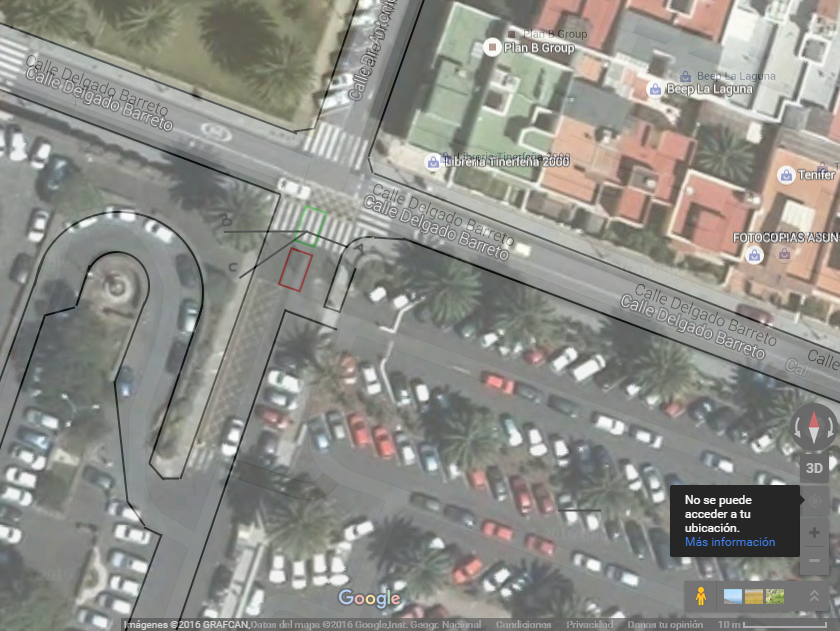
\includegraphics[width=140mm,height=120mm]{Parking}
	\label{fig:parking}
	\caption{Se puede apreciar la estructura del parking central. Los puntos A, B y C señalan las posiciones de los beacons.}
\end{figure}

\subsubsection{Funcionamiento}


En cuanto se accede al módulo de parking de \textit{BulletPoint}, la aplicación muestra una lista con los diferentes parkings y el número de plazas de cada recinto. Esta lista se obtiene mediante una consulta a una API diseñada en colaboración con Alberto Morales, quien se ha encargado de configurar el servicio para facilitar a la aplicación la información necesaria. De la lista de parkings, el usuario ha de seleccionar al que quiere acceder, identificando así la imagen y zonas a dibujar. Esta selección da paso a un escáner que comienza a detectar la posición del usuario y a situarlo en la imagen. Si el usuario se encuentra en una de las zonas designadas para entrar o salir del parking, se lanzará la acción, que en este caso consiste en una petición de apertura contra el servidor. En este caso cada zona posee un identificador de barrera que es el que usa la petición para determinar que barrera debe abrir. 


Por otro lado esta petición debe ir autentificada, para poder acceder, por lo que la aplicación ha negociado previamente un secreto con el servidor que la identifica y le permite realizar la acción de apertura utilizando un número identificativo basado en la MAC del dispositivo de pruebas.


\subsubsection{Dificultades}

En este caso de uso las dificultades han radicado en el hecho de comunicarse con el servidor para realizar las llamadas. La trilateración se ha realizado de la misma manera por lo que no ha habido grandes problemas. Además de estas dificultades, cabe añadir una adicional y es que la seguridad del parking depende del sistema single log in de la ULL, por lo que ha habido que buscar la manera de abordar este tema. Sin embargo, Alberto Morales se ha implicado en todo momento intentado resolver las necesidades de la aplicación de manera óptima, lo que ha sido una gran ayuda.

\subsubsection{Ampliación}

Para ampliar este caso de uso se deberían incluir nuevos beacons, 3 mínimo por cada recinto, nuevas imagenes de las localizaciones (exteriores o interiores) y nuevas áreas; Las áreas serían esenciales para definir las acciones de apertura de las barreas. Si las zonas acaban siendo muchas, sería recomendable crear una base de datos  para almacenar las localizaciones, las zonas y las imágenes a cargar.

\section{Despliegue}

El despliegue de estos dispositivos es variable como hemos podido comprobar con los distintos casos de uso. Sin embargo hay ciertas consideraciones comunes a en todos los casos, si lo que deseamos es un sistema que detecte entradas y salidas, independientemente de la posición exacta del usuario, simplemente necesitaremos un único beacon como regla general. 


Sin embargo, si se pretende conocer la localización más precisa del usuario necesitaremos recurir a un método como la trilateración \cite{URL::trilateracion}. Serán necesarios un mínimo de 3 beacons. Incrementando el número de beacons es posible aumentar la precisión con la que se percibe la posición del usuario. El algoritmo no es totalmente exacto, puesto que depende de las distancias calculadas a los beacons, sin embargo estas distancias pueden variar. Existen diversos factores que pueden influir en la calidad de la señal del Bluetooth y por tanto distorsionar estas distancias, entre otros factores podemos destacar principalmente:


\begin{itemize}
\item Físicos:  paredes, personas o elementos del entorno principalmente.
\item Intangibles: interferencias con otras ondas.
\item Configurables: la intensidad de la señal y por tanto su rango es configurable.
\end{itemize}


Todos estos factores han de ser tomados en cuenta a la hora de realizar el despligue de los beacons. Otro factor a tener en cuenta es la altura. Los dispositivos es recomendables levantarlos cierta altura sobre el nivel del suelo. A la hora de probarlos se ha intentado, en la medida de lo posible, mantenerlos a un nivel elevado sobre la altura de las personas y siempre intentando mantener esta medida de altura para los diferentes beacons. En cuanto al despliegue de la aplicación, el código fuente de BulletPoint se encuentra disponible para su descarga en \cite{URL::repositorioAplicacion}, bajo licencia Creative Commons Reconocimiento-NoComercial-CompartirIgual 4.0 Internacional \cite{URL::licencia}.






% ---------------------------------------------------
%
% Trabajo de Fin de Grado. 
% Author: Laura Padrón Jorge. 
% Capítulo: La aplicacion BulletPoint. 
% Fichero: Cap4_TheApplication.tex
%
% ----------------------------------------------------
%

\chapter{La aplicación BulletPoint} \label{chap:laaplicacion} 

En este capítulo trataremos diversos temas relacionados con la aplicación, comenzaremos por definir posibles casos de uso en el ámbito universitario, tocaremos diversos temas relacionados incluyendo dificultades durante el desarrollo y acabaremos discutiendo posibles líneas futuras de desarrollo.

 
\section{Aplicaciones móviles en entornos universitarios}


Actualmente las posibilidades de las aplicaciones móviles para entornos universitarios se presentan amplias, cada universidad intenta tener su propia aplicación siguiendo un patrón similar. Realizando una investigación general de las aplicaciones disponibles en el mercado observamos que estas aplicaciones se centran en ofrecer servicios propios (servicio de correo, moodle, chat entre usuarios,etc), mantener al alumno informado y agilizarle los trámites principalmente. 

En un principio, estas aplicaciones se centraban en atraer alumnos, centrandose en la calidad de la universidad y mostrando las posibilidades que ofrecían, sin embargo con el paso de los años y el desarrollo creciente de las aplicaciones móviles, se muestra un cambio en esta estrategia. Ahora las aplicaciones tienen una doble función, no sólo buscan el acceso de nuevos estudiantes sino que también intentan mejorar la experiencia de los alumnos existentes y acercar a los nuevos a la experiencia de la universidad. 

Algunos ejemplos posibles los encontramos en el marketplace de google:

%No se si se pueden poner imagenes de aplicaciones universitarias en el marketplace.

Uno de los hechos que podemos observar es que las universidades están intentando obtener una solución rápida para desarrollar su app, una de las soluciones que se suelen adoptar es la creación de plantillas web optimizadas de su sitio web, lo que podemos considerar una opción rápida con un coste bajo.

En un futuro próximo con la aparición de los beacons, nos surge la pregunta ¿ Serán capaces estos dispositivos de transformar la educación ? De acuerdo con una encuesta realizado por %\textit{Software and Information Industry Association (SIAA)} \citeURL::SIAA%, casi todos los estudiantes hoy en día tienen acceso a un dispositivo móvil a través de %\textit{BYOD} \citeURL::BYOD%.El acercamiento de los estudiantes a los dispositivos móviles ha abierto la puerta a esta nueva tecnología.

\section {Posibles casos de uso de la tecnología beacon en entornos universitarios}

Como mencionaba antes, una de las posibilidades que se presentan para explotar esta tecnología se encuentra en las instituciones de enseñanza, las cuales podrían utilizar los beacons para facilitar a sus alumnos, profesores y demás personal involucrado  una serie de servicios de gran utilidad.

Sin embargo, para utilizar esta tecnología es necesario cumplir una serie de condiciones:

\begin{itemize}
\item Tener instalada la aplicación en su dispositivo móvil.
\item Tener activado el bluetooth.
\item La aplicación ha de estar despierta.
\item Las beacons han de estar desplegadas y configuradas correctamente en lugares clave donde el rango sea óptimo.
\end{itemize}

En el caso de dispositivos Apple no es necesario tener activado el bluetooth ya que el SO se encarga de captar las señales BLE, aparte tampoco es necesario que la app esté despierta ya que nuevamente el SO se encarga de despertar a la aplicación involucrada. Sin embargo Apple no ha desarrollado un IBeacon físico aún, aunque en un futuro, se espera que sus dispositivos móviles puedan funcionar como un beacon bidirecional.


Asimismo podemos afirmar que prácticamente hoy en día la mayoría de las universidades cuentan con una disposición amplia en los que se refiere a servicios y despliegue de medios. Como ejemplo podemos coger la Universidad de la Laguna, la cual cuenta con una red WiFi con un rango de cobertura casi completo de sus instalaciones y una amplia carta de servicios disponibles para sus alumnos. Además cuenta con una serie de dispositivos beacons facilitados, que podrían ser instalados adecuadamente en lugares estratégicos. 

Partiendo de esta base, procederemos a explorar posibles casos de uso para los beacons en entornos universitarios como referente:

\subsection{Guía a través del Campus de la Universidad}

Este caso de uso cubre la funcionalidad destacada de un beacon, el posicionamiento y guia tanto en exteriores como en interiores. 

Como interesados podríamos destacar: 

\begin{itemize}
\item Personal invitado a jornadas o eventos en instalaciones de la Universidad.
\item Alumnos de intercambio en programas internacionales.
\item Alumnos de nuevo acceso.
\item Personas con discapacidad.
\end{itemize}

\begin{figure}[h]
	\centering
	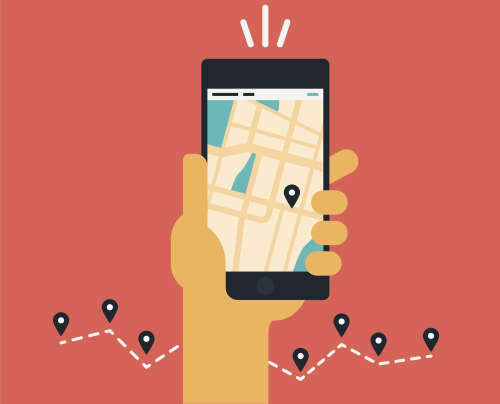
\includegraphics[width=\columnwidth]{locationMobileBeacon}
	\caption{Servicios de localización a través de la Universidad}
	\label{fig:beaconLocation}
\end{figure}

El funcionamiento sería el siguiente: 

El usuario transita por las inmediaciones del campus universitario. En cuanto entra el el rango delimitado por el beacon, su movil vibra. El usuario mira su móvil y ha recibido una notificación de la aplicación de la Universidad. La notificación le informa que ha entrado en el rango del campus y si quiere entrar al sistema de navegación. Si el usuario acepta, la aplicación le muestra el camino mostrándole en todo momento su ubicación como un punto de color sobre el mapa de la ULL. Este mapa tiene marcados puntos de interés que contienen información de diferente tipo dependiendo del punto marcado: nombre, historia, página web, teléfono de contacto, trámites asociados son algunos de los datos que podría mostrar. El mapa se va actualizando dependiendo de la posición del usuario permitiendo volver a la vista más alejada en cualquier momento para una visualización más general.


\subsection{Descarga automática de material}

Este caso de uso resultaría muy útil para personal lectivo y para estudiantes, los cuales accederían de manera más sencilla al material dado. También sería aplicable para ponientes de charlas los cuales no tendrían que colgar sus apuntes en alguna plataforma externa o llevarlos consigo en  un almacenamiento externo para compartirlo al finalizar.

El funcionamiento sería el siguiente: 

El profesor o poniente lleva consigo un beacon y sus estudiantes u oyentes tienen instalados en sus dispositivos la aplicación. El profesor es capaz de introducir en su aplicación con el perfil de profesor (el poniente con su correspondiente perfil), indicaciones del material a utilizar en el evento. El profesor carga consigo el pequeño dispositivo e indica a sus alumnos que conecten el bluetooth y abran la aplicación, al entrar en el rango, la aplicación pedira permiso al alumno para descargarse el contenido indicado por el profesor. Si el alumno acepta, la aplicación pasaría a abrir  el contenido indicado por la página correspondiente.


\subsection{Acceso al parking y conteo de número de vehículos estacionados}


Este caso de uso proporcionaría información muy útil a los usuarios del parking de la universidad, informando del número coches estacionados en el parking y de las plazas restantes a ocupar en tiempo real.

El funcionamiento sería el siguiente: 

El personal de la Ull tendría la aplicación en su móvil, al acercarse a la barra del parking, el usuario activaría el bluetooth de su móvil. El beacon por su parte registraría un nuevo punto entrando en el rango de acción del parking. La aplicación comprobaría que el usuario está autorizado a entrar en el parking y procedería a abrir la puerta del parking dejando entrar al vehículo. Cuando el vehículo saliese del rango del beacon por el rango interior, la aplicación registraría entonces un nuevo acceso al parking y contabilizaría otro vehículo dentro de parking. Al salir del parking el proceso sería el mismo, por lo tanto la aplicación sería capaz de informar al usuario de las plazas ocupadas en tiempo real.


\subsection{Gestión de eventos e información, entrada automática}

El funcionamiento sería el siguiente: 

Los alumnos transitan los interiores de la Universidad de camino a sus clases. Los beacons están desplegados en las inmediaciones de lugares de interés, tipo aularium, paraninfo, clases que se utilicen a modo de salas de reuniones o seminarios. Al pasar por las inmediaciones de estos lugares de interés la aplicación alertaría al usuario de eventos que se celebrán en esos lugares, proporcionandole información de diversa índole, ponientes, tema de la charla, acceso, teléfono de contacto o otra información similar.  Al mismo tiempo la aplicación también cuenta con un tablón donde se muestran posibles eventos futuros. Estos eventos pueden ser muy variados y corresponder a diferentes tipos de actividades. Al mismo tiempo se podría confirmar la entrada al evento en el caso de haberla, mediante un código de acceso identificativo generado al realizar el pago del evento.

\begin{figure}[H]
	\centering
	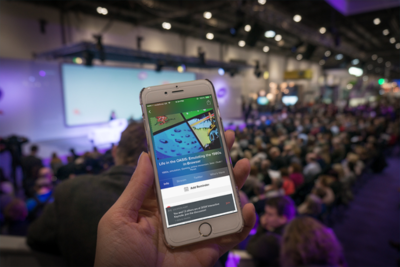
\includegraphics[width=\columnwidth]{BeaconEvent}
	\label{fig:eventBeacon}
\end{figure}

\subsection{Despacho del profesorado e información}

El funcionamiento podría abarcarse de dos maneras, por un lado, podría utilizarse para proveer a los alumnos de información acerca del grupo de despachos, aclarando que profesores tienen el despacho en la zona, horario de tutorías, correo electrónico de contacto, horario de corrección de exámenes, etc. De esta manera el alumno al acercarse a la zona sería capaz de saber información de todos los profesores, o si busca uno en particular la aplicación le da la opción de elegir su nombre de una lista y simplemente comprobar si tiene su despacho en esa zona. 

Por otro lado, este caso de uso podría abarcarse para proporcionar una información adicional, comprobando si el profesor está en la zona en ese momento y se encuentra disponible. El profesor tendrá un perfil de la aplicación con un código identificativo que le distingue de los demás profesores. Estos datos se guardarían en un servicio externo, y el beacon sería el encargado de registrar las entradas y salidas de los profesores. En cuanto al estado de disponibilidad, sería un dato que actualizaría el profesor desde su perfil de profesor en la aplicación. Los alumnos recibirían estos estados desde su lado de la aplicación y serían capaces de saber cuando el profesor se encuentra disponible mediante la aplicación. 

\subsection{Información y descuentos para usuarios de la APP}

Este caso de uso no solo dependería de la universidad sino de establecimientos comerciales interesados. La idea sería la siguiente: 

La universidad en colaboración con un establecimiento comercial le entrega un beacon. La aplicación contaría con un perfil para el dueño del establecimiento, donde sería capaz de introducir información que quiere que se muestre al usuario al pasar cerca de su establecimiento, mensajes de información, descuentos u ofertas especiales por ejemplo. El usuario al pasar por las inmediaciones del establecimeinto recibe en su aplicación una notificación del establecimiento con la información introducida por el dueño anteriormente. Al aceptar la notificación el usuario podría ser redirigido a la página web del establecimiento por ejemplo, para ver la oferta mejor o simplemente descartarla. En cualquier caso el establecimiento ha conseguido captar la atención de un posible cliente, y el usuario se benefiaría de ofertas y descuentos. 

\subsection{Control de asistencia}

Este caso de uso podría ir ligado al de Descarga automática de material, el funcionamiento sería el siguiente: 

El alumno conectaría el bluetooth de su móvil al iniciar la clase, en este momento la aplicación detectaría los dispositivos con los identificadores de alu de los alumnos y los dejaría registrados a la clase en el horario establecido. Los profesores serían capaces en todo momento desde su perfil de profesor de consultar asistencia. Si lo unimos con la descarga atomática de material proporcionaría comodidad tanto a alumnos como a profesores. Sin embargo un impedimento podría ser el rango del beacon o la necesidad de activar el bluetooth, ya que si  no tienes batería tendría que haber  un método secundario igualmente. 

\subsection{Control de acceso a instalaciones}

En control de acceso a las aulas y edificios puede ser un tema abordable mediante el uso de estos dispositivos, los lectores de tarjetas pasarían a ser algo innecesario. El alumno simplemente tendría que activar el bluetooth cerca del punto de acceso, se comprobaría su identificador y procedería a darle a acceso o a informarle de su falta de permiso para acceder. El acceso a estos puntos podría quedar guardado en algún tipo de plataforma donde se monitorizen los accesos dependiendo de la seguridad de acceso al aula.

\subsection{Biblioteca Informativa}

Otro posible uso que se le podría dar a esta tecnología tiene que ver con las bibliotecas o lugares de almacenamiento de material. El alumno se acercaría a la biblioteca buscando un libro específico, en la aplicación estaría registrado la localización de los libros disponibles en los estantes, lo que le indicaría al alumno la posición del libro que busca. Para lugares amplios donde hay gran cantidad de material incluso podría guiar al usuario como un punto por las instalaciones hasta llegar a su objetivo, informarle de si quedan ejemplares disponibles o de fecha prevista de entrada de algún material, de esta manera el alumno agilizaría su búsqueda en gran medida.

\begin{figure}[H]
	\centering
	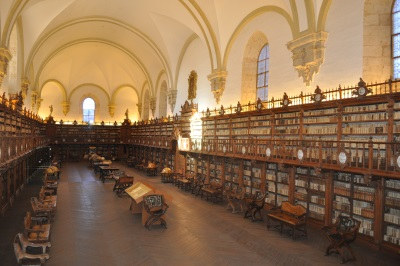
\includegraphics[width=\columnwidth]{BibliotecaSalamanca}
	\caption{La biblioteca de la Universidad de Salamanca (USAL) contiene más de 1.000.000 de ejemplares lo que puede hacer dificil la localización de algunos títulos.}
	\label{fig:bibliotecaUSAL}
\end{figure}

\subsection{Actividades interactivas por el Campus, jornadas de acogida u otros eventos}

En un aspecto más recreativo, se podría tener en cuenta el uso de los beacons para organizar juegos o actividades divertidas para los alumnos. Estos eventos dependerían de los organizadores, pero podrían consistir en alguna actividad que implicase movimiento y colaboración. Los alumnos tendrían que registrarse con su identificador, una ruta a través del campus con adivinanzas o puzzles que tengan que ver con diferentes temáticas por ejemplo fomentaría a los alumnos a trabajar en equipo y utilizar su ingenio.Al mismo tiempo se podría aplicar algún tipo de recompensa para los ganadores, descuentos o bonos tramitados por medio de la aplicación, lo que fomentaría la participación estudiantil.

\section{4 Casos de uso elegidos}



\section{Despliegue}



% ---------------------------------------------------
%
% Trabajo de Fin de Grado. 
% Author: Laura Padrón Jorge. 
% Capítulo: La aplicacion BulletPoint. 
% Fichero: Cap4_TheApplication.tex
%
% ----------------------------------------------------
%

\chapter{La aplicación BulletPoint} \label{chap:laaplicacion} 

En este capítulo trataremos diversos temas relacionados con la aplicación, comenzaremos por definir posibles casos de uso en el ámbito universitario, tocaremos diversos temas relacionados incluyendo dificultades durante el desarrollo y acabaremos discutiendo posibles líneas futuras de desarrollo.

 
\section{Aplicaciones móviles en entornos universitarios}


Actualmente las posibilidades de las aplicaciones móviles para entornos universitarios se presentan amplias, cada universidad intenta tener su propia aplicación siguiendo un patrón similar. Realizando una investigación general de las aplicaciones disponibles en el mercado observamos que estas aplicaciones se centran en ofrecer servicios propios (servicio de correo, moodle, chat entre usuarios,etc), mantener al alumno informado y agilizarle los trámites principalmente. 

En un principio, estas aplicaciones se centraban en atraer alumnos, centrandose en la calidad de la universidad y mostrando las posibilidades que ofrecían, sin embargo con el paso de los años y el desarrollo creciente de las aplicaciones móviles, se muestra un cambio en esta estrategia. Ahora las aplicaciones tienen una doble función, no sólo buscan el acceso de nuevos estudiantes sino que también intentan mejorar la experiencia de los alumnos existentes y acercar a los nuevos a la experiencia de la universidad. 

Algunos ejemplos posibles los encontramos en el marketplace de google:

%No se si se pueden poner imagenes de aplicaciones universitarias en el marketplace.

Uno de los hechos que podemos observar es que las universidades están intentando obtener una solución rápida para desarrollar su app, una de las soluciones que se suelen adoptar es la creación de plantillas web optimizadas de su sitio web, lo que podemos considerar una opción rápida con un coste bajo.

En un futuro próximo con la aparición de los beacons, nos surge la pregunta ¿ Serán capaces estos dispositivos de transformar la educación ? De acuerdo con una encuesta realizado por %\textit{Software and Information Industry Association (SIAA)} \citeURL::SIAA%, casi todos los estudiantes hoy en día tienen acceso a un dispositivo móvil a través de %\textit{BYOD} \citeURL::BYOD%.El acercamiento de los estudiantes a los dispositivos móviles ha abierto la puerta a esta nueva tecnología.

\section {Posibles casos de uso de la tecnología beacon en entornos universitarios}

Como mencionaba antes, una de las posibilidades que se presentan para explotar esta tecnología se encuentra en las instituciones de enseñanza, las cuales podrían utilizar los beacons para facilitar a sus alumnos, profesores y demás personal involucrado  una serie de servicios de gran utilidad.

Sin embargo, para utilizar esta tecnología es necesario cumplir una serie de condiciones:

\begin{itemize}
\item Tener instalada la aplicación en su dispositivo móvil.
\item Tener activado el bluetooth.
\item La aplicación ha de estar despierta.
\item Las beacons han de estar desplegadas y configuradas correctamente en lugares clave donde el rango sea óptimo.
\end{itemize}

En el caso de dispositivos Apple no es necesario tener activado el bluetooth ya que el SO se encarga de captar las señales BLE, aparte tampoco es necesario que la app esté despierta ya que nuevamente el SO se encarga de despertar a la aplicación involucrada. Sin embargo Apple no ha desarrollado un IBeacon físico aún, aunque en un futuro, se espera que sus dispositivos móviles puedan funcionar como un beacon bidirecional.


Asimismo podemos afirmar que prácticamente hoy en día la mayoría de las universidades cuentan con una disposición amplia en los que se refiere a servicios y despliegue de medios. Como ejemplo podemos coger la Universidad de la Laguna, la cual cuenta con una red WiFi con un rango de cobertura casi completo de sus instalaciones y una amplia carta de servicios disponibles para sus alumnos. Además cuenta con una serie de dispositivos beacons facilitados, que podrían ser instalados adecuadamente en lugares estratégicos. 

Partiendo de esta base, procederemos a explorar posibles casos de uso para los beacons en entornos universitarios como referente:

\subsection{Guía a través del Campus de la Universidad}

Este caso de uso cubre la funcionalidad destacada de un beacon, el posicionamiento y guia tanto en exteriores como en interiores. 

Como interesados podríamos destacar: 

\begin{itemize}
\item Personal invitado a jornadas o eventos en instalaciones de la Universidad.
\item Alumnos de intercambio en programas internacionales.
\item Alumnos de nuevo acceso.
\item Personas con discapacidad.
\end{itemize}

\begin{figure}[h]
	\centering
	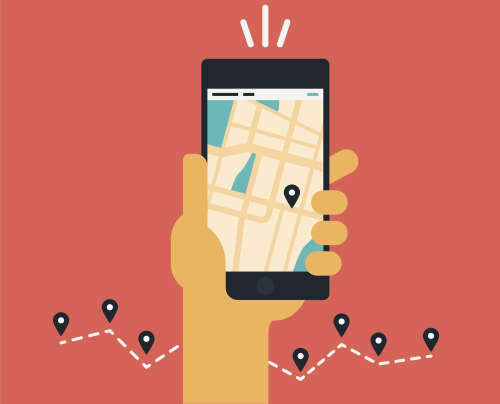
\includegraphics[width=\columnwidth]{locationMobileBeacon}
	\caption{Servicios de localización a través de la Universidad}
	\label{fig:beaconLocation}
\end{figure}

El funcionamiento sería el siguiente: 

El usuario transita por las inmediaciones del campus universitario. En cuanto entra el el rango delimitado por el beacon, su movil vibra. El usuario mira su móvil y ha recibido una notificación de la aplicación de la Universidad. La notificación le informa que ha entrado en el rango del campus y si quiere entrar al sistema de navegación. Si el usuario acepta, la aplicación le muestra el camino mostrándole en todo momento su ubicación como un punto de color sobre el mapa de la ULL. Este mapa tiene marcados puntos de interés que contienen información de diferente tipo dependiendo del punto marcado: nombre, historia, página web, teléfono de contacto, trámites asociados son algunos de los datos que podría mostrar. El mapa se va actualizando dependiendo de la posición del usuario permitiendo volver a la vista más alejada en cualquier momento para una visualización más general.


\subsection{Descarga automática de material}

Este caso de uso resultaría muy útil para personal lectivo y para estudiantes, los cuales accederían de manera más sencilla al material dado. También sería aplicable para ponientes de charlas los cuales no tendrían que colgar sus apuntes en alguna plataforma externa o llevarlos consigo en  un almacenamiento externo para compartirlo al finalizar.

El funcionamiento sería el siguiente: 

El profesor o poniente lleva consigo un beacon y sus estudiantes u oyentes tienen instalados en sus dispositivos la aplicación. El profesor es capaz de introducir en su aplicación con el perfil de profesor (el poniente con su correspondiente perfil), indicaciones del material a utilizar en el evento. El profesor carga consigo el pequeño dispositivo e indica a sus alumnos que conecten el bluetooth y abran la aplicación, al entrar en el rango, la aplicación pedira permiso al alumno para descargarse el contenido indicado por el profesor. Si el alumno acepta, la aplicación pasaría a abrir  el contenido indicado por la página correspondiente.


\subsection{Acceso al parking y conteo de número de vehículos estacionados}


Este caso de uso proporcionaría información muy útil a los usuarios del parking de la universidad, informando del número coches estacionados en el parking y de las plazas restantes a ocupar en tiempo real.

El funcionamiento sería el siguiente: 

El personal de la Ull tendría la aplicación en su móvil, al acercarse a la barra del parking, el usuario activaría el bluetooth de su móvil. El beacon por su parte registraría un nuevo punto entrando en el rango de acción del parking. La aplicación comprobaría que el usuario está autorizado a entrar en el parking y procedería a abrir la puerta del parking dejando entrar al vehículo. Cuando el vehículo saliese del rango del beacon por el rango interior, la aplicación registraría entonces un nuevo acceso al parking y contabilizaría otro vehículo dentro de parking. Al salir del parking el proceso sería el mismo, por lo tanto la aplicación sería capaz de informar al usuario de las plazas ocupadas en tiempo real.


\subsection{Gestión de eventos e información, entrada automática}

El funcionamiento sería el siguiente: 

Los alumnos transitan los interiores de la Universidad de camino a sus clases. Los beacons están desplegados en las inmediaciones de lugares de interés, tipo aularium, paraninfo, clases que se utilicen a modo de salas de reuniones o seminarios. Al pasar por las inmediaciones de estos lugares de interés la aplicación alertaría al usuario de eventos que se celebrán en esos lugares, proporcionandole información de diversa índole, ponientes, tema de la charla, acceso, teléfono de contacto o otra información similar.  Al mismo tiempo la aplicación también cuenta con un tablón donde se muestran posibles eventos futuros. Estos eventos pueden ser muy variados y corresponder a diferentes tipos de actividades. Al mismo tiempo se podría confirmar la entrada al evento en el caso de haberla, mediante un código de acceso identificativo generado al realizar el pago del evento.

\begin{figure}[H]
	\centering
	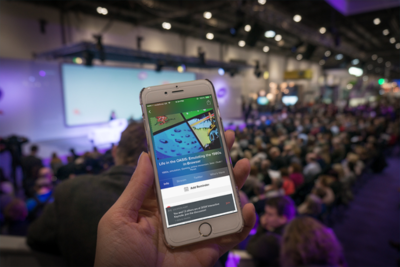
\includegraphics[width=\columnwidth]{BeaconEvent}
	\label{fig:eventBeacon}
\end{figure}

\subsection{Despacho del profesorado e información}

El funcionamiento podría abarcarse de dos maneras, por un lado, podría utilizarse para proveer a los alumnos de información acerca del grupo de despachos, aclarando que profesores tienen el despacho en la zona, horario de tutorías, correo electrónico de contacto, horario de corrección de exámenes, etc. De esta manera el alumno al acercarse a la zona sería capaz de saber información de todos los profesores, o si busca uno en particular la aplicación le da la opción de elegir su nombre de una lista y simplemente comprobar si tiene su despacho en esa zona. 

Por otro lado, este caso de uso podría abarcarse para proporcionar una información adicional, comprobando si el profesor está en la zona en ese momento y se encuentra disponible. El profesor tendrá un perfil de la aplicación con un código identificativo que le distingue de los demás profesores. Estos datos se guardarían en un servicio externo, y el beacon sería el encargado de registrar las entradas y salidas de los profesores. En cuanto al estado de disponibilidad, sería un dato que actualizaría el profesor desde su perfil de profesor en la aplicación. Los alumnos recibirían estos estados desde su lado de la aplicación y serían capaces de saber cuando el profesor se encuentra disponible mediante la aplicación. 

\subsection{Información y descuentos para usuarios de la APP}

Este caso de uso no solo dependería de la universidad sino de establecimientos comerciales interesados. La idea sería la siguiente: 

La universidad en colaboración con un establecimiento comercial le entrega un beacon. La aplicación contaría con un perfil para el dueño del establecimiento, donde sería capaz de introducir información que quiere que se muestre al usuario al pasar cerca de su establecimiento, mensajes de información, descuentos u ofertas especiales por ejemplo. El usuario al pasar por las inmediaciones del establecimeinto recibe en su aplicación una notificación del establecimiento con la información introducida por el dueño anteriormente. Al aceptar la notificación el usuario podría ser redirigido a la página web del establecimiento por ejemplo, para ver la oferta mejor o simplemente descartarla. En cualquier caso el establecimiento ha conseguido captar la atención de un posible cliente, y el usuario se benefiaría de ofertas y descuentos. 

\subsection{Control de asistencia}

Este caso de uso podría ir ligado al de Descarga automática de material, el funcionamiento sería el siguiente: 

El alumno conectaría el bluetooth de su móvil al iniciar la clase, en este momento la aplicación detectaría los dispositivos con los identificadores de alu de los alumnos y los dejaría registrados a la clase en el horario establecido. Los profesores serían capaces en todo momento desde su perfil de profesor de consultar asistencia. Si lo unimos con la descarga atomática de material proporcionaría comodidad tanto a alumnos como a profesores. Sin embargo un impedimento podría ser el rango del beacon o la necesidad de activar el bluetooth, ya que si  no tienes batería tendría que haber  un método secundario igualmente. 

\subsection{Control de acceso a instalaciones}

En control de acceso a las aulas y edificios puede ser un tema abordable mediante el uso de estos dispositivos, los lectores de tarjetas pasarían a ser algo innecesario. El alumno simplemente tendría que activar el bluetooth cerca del punto de acceso, se comprobaría su identificador y procedería a darle a acceso o a informarle de su falta de permiso para acceder. El acceso a estos puntos podría quedar guardado en algún tipo de plataforma donde se monitorizen los accesos dependiendo de la seguridad de acceso al aula.

\subsection{Biblioteca Informativa}

Otro posible uso que se le podría dar a esta tecnología tiene que ver con las bibliotecas o lugares de almacenamiento de material. El alumno se acercaría a la biblioteca buscando un libro específico, en la aplicación estaría registrado la localización de los libros disponibles en los estantes, lo que le indicaría al alumno la posición del libro que busca. Para lugares amplios donde hay gran cantidad de material incluso podría guiar al usuario como un punto por las instalaciones hasta llegar a su objetivo, informarle de si quedan ejemplares disponibles o de fecha prevista de entrada de algún material, de esta manera el alumno agilizaría su búsqueda en gran medida.

\begin{figure}[H]
	\centering
	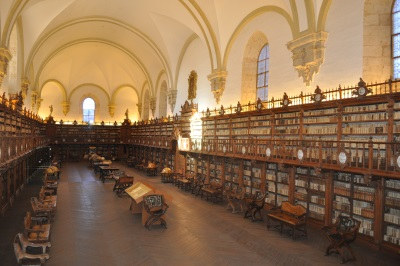
\includegraphics[width=\columnwidth]{BibliotecaSalamanca}
	\caption{La biblioteca de la Universidad de Salamanca (USAL) contiene más de 1.000.000 de ejemplares lo que puede hacer dificil la localización de algunos títulos.}
	\label{fig:bibliotecaUSAL}
\end{figure}

\subsection{Actividades interactivas por el Campus, jornadas de acogida u otros eventos}

En un aspecto más recreativo, se podría tener en cuenta el uso de los beacons para organizar juegos o actividades divertidas para los alumnos. Estos eventos dependerían de los organizadores, pero podrían consistir en alguna actividad que implicase movimiento y colaboración. Los alumnos tendrían que registrarse con su identificador, una ruta a través del campus con adivinanzas o puzzles que tengan que ver con diferentes temáticas por ejemplo fomentaría a los alumnos a trabajar en equipo y utilizar su ingenio.Al mismo tiempo se podría aplicar algún tipo de recompensa para los ganadores, descuentos o bonos tramitados por medio de la aplicación, lo que fomentaría la participación estudiantil.

\section{4 Casos de uso elegidos}



\section{Despliegue}




%\newpage{\pagestyle{empty}}
%\thispagestyle{empty}

%\chapter{Presupuesto}
%\label{chapter:Presupuesto}

%\input{cap7.tex}

%%%%%%%%%%%%%%%%%%%%%%%%%%%%%%%%%%%%%%%%%%%%%%%%%%%%%%%%%%%%%%%%%%%%%%%%%%%%%%%

%%%%%%%%%%%%%%%%%%%%%%%%%%%%%%%%%%%%%%%%%%%%%%%%%%%%%%%%%%%%%%%%%%%%%%%%%%%%%%%
%\newpage{\pagestyle{empty}}
%\thispagestyle{empty}
%\begin{appendix}
%
%\chapter{Título del Apéndice 1}
%\label{appendix:1}
%\input{apendice1.tex}
%
%\chapter{Título del Apéndice 2}
%\label{appendix:2}
%\input{apendice2.tex}
%
%\end{appendix}
%%%%%%%%%%%%%%%%%%%%%%%%%%%%%%%%%%%%%%%%%%%%%%%%%%%%%%%%%%%%%%%%%%%%%%%%%%%%%%%
\addcontentsline{toc}{chapter}{Bibliografía}
%\bibliographystyle{plain}
\bibliographystyle{bmc_article} 
\renewcommand{\bibname}{Bibliografía}   %  Para que no aparezca Índice de figuras
\bibliography{bibliografia}

%%%%%%%%%%%%%%%%%%%%%%%%%%%%%%%%%%%%%%%%%%%%%%%%%%%%%%%%%%%%%%%%%%%%%%%%%%%%%%%

\end{document}
